\ssection[Sammendrag]{Sammendrag}

\begin{multicols}{2}
% New executive summary for Norwegian in Norwegian bokmål
Informasjonsteknologi påvirker hverdagen vår. Vi bruker datamaskiner når vi skriver, redigerer, regner ut, søker etter informasjon, og i økende grad også når vi leser, hører på musikk, ser på bilder og ser film. Vi har med oss små datamaskiner i lomma og bruker disse til å ringe, skrive e-post, innhente informasjon og til å underholde oss selv hvor vi enn er. Men hvilken innvirkning har denne utstrakte digitaliseringen av informasjon, kunnskap og daglig kommunikasjon på språket vårt? Vil språket vårt endre seg eller til og med forsvinne? Hva er sjansene for at norsk språk vil bestå?        

Mange av de 6000 språkene som finnes i verden i dag vil ikke overleve i det globaliserte digitale informasjonssamfunnet. En regner med at minst 2000 språk kommer til å forsvinne de kommende tiårene.  Andre vil fremdeles spille en rolle i privatsfæren og lokalsamfunnet, men ikke i det bredere offentlige liv som næringsliv og akademia. Statusen til et språk avhenger ikke bare av tallet på brukere eller hvor mange bøker, filmer og TV-stasjoner som benytter språket, men også av i hvilken grad språket gjør seg gjeldende i den digitale virkeligheten og brukes  i programvareapplikasjoner. 

I denne sammenhengen sliter norsk fremdeles med voksesmerter. I begynnelsen av det tjueførste århundret eksisterte norsk språkteknologi bare i svært liten skala. Det fantes et relativt godt system for oversettelse fra bokmål og nynorsk, der var stavekontroll, og det fantes også et lite dialogsystem som svarer på spørsmål, mens folk flest lo av den dårlige kvaliteten til de første talegjenkjenningsprogrammene. Et ambisiøst industrielt initiativ til språkteknologiutvikling på Voss mislyktes. Innen høyere utdanning fantes det program for språkteknologi og datalingvistikk, og det eksisterte forskning på disse feltene, men det manglet språkressurser og språkverktøy.            

Bildet endret seg da forskningsrådet tok initiativ til et språkteknologiprogram i 2002, med sikte på å utvikle ny kunnskap og nødvendige verktøy. Programmet resulterte i flere prosjekt som skapte ny kompetanse og et bedre grunnlag for norsk språkteknologi. De største prosjektene i dette språkteknologiprogrammet leverte et tekst-til-tale-system og en demonstrator for oversettelse av høy kvalitet fra norsk til engelsk.

Etter Stortingsmeldingen fra 2008 \cite{stm35:2008}, og vedtaket av denne meldingen i Stortinget, ble en fritt tilgjengelig samling av norske språkteknologiske ressurser, \emph{Språkbanken}, etablert i 2010. Språkbanken er nå i gang med å bygge opp og distribuere norske språkdata, en oppgave som lenge har vært etterspurt innen forskning og utvikling. Dersom dette arbeidet blir opprettholdt, vil det utgjøre en uvurderlig investering i norsk språks fremtid.     

På tross av en betydelig utvikling innen norsk språkteknologi det siste tiåret viser denne rapporten at det ennå bare er for basisverktøy og -ressurser at situasjonen er noenlunde tilfredsstillende. Når det gjelder mer avanserte applikasjoner, finnes det fremdeles svært få verktøy og ressurser for norsk, og vi har fremdeles langt igjen før norsk språk er sikret en fremtid som fullverdig aktør i det moderne -- og framtidige -- europeiske språksamfunnet.   

Informasjons- og kommunikasjonsteknologien forbereder seg nå til neste teknologirevolusjon. I kjølvannet av personlige datamaskiner, nettverk, stadig mindre og lettere komponenter, multimedia, mobile enheter og databehandling i digitale skyer, vil den neste generasjonen teknologi bestå av programvare som ikke bare forstår talte og skrevne bokstaver og lyder, men også hele ord og setninger, og som støtter brukeren bedre enn dagens teknologi, fordi den snakker, kjenner og forstår språket deres. Forløpere i denne utviklingen er IBMs superdatamaskin Watson, som slo USA-mesteren i kunnskapsspillet “Jeopardy”, og Apples mobilassistent Siri for iPhone, som responderer på språkkommandoer og kan svare på spørsmål på engelsk, tysk, fransk og japansk. Et norsk talegjenkjenningssystem for iPhone er tilgjengelig, men det er fremdeles mye mindre pålitelig enn det tilsvarende engelske systemet. 

Språkbrukere kommuniserer allerede ved hjelp av teknologien som er utviklet for deres språk. Etter hvert vil teknologiske innretninger, som respons på enkle talekommandoer, være i stand til å hente de viktigste nyhetene og informasjonen fra den globale digitale kunnskapsbasen. Språkbasert teknologi vil kunne oversette automatisk eller fungere som støtte for tolker, lage sammendrag av samtaler og dokumenter og være et hjelpemiddel i læringssituasjoner. Språkteknologi vil for eksempel kunne hjelpe innvandrere med å lære norsk, og dermed også med integrering i det norske samfunnet.        
 
Informasjons- og kommunikasjonsteknologi vil gjøre industrielle roboter og tjenesteroboter (som i dag er under utvikling i forskningslaboratorier) i stand til å forstå hva brukeren ønsker at de skal gjøre og å rapportere om oppgavene de har utført. Et slikt prestasjonsnivå strekker seg langt ut over enkle bokstavlister og leksikon, stavekontroller og uttaleregler. Skal språkteknologi kunne tolke spørsmål og levere utfyllende og relevante svar, må den bevege seg fra basale tilnærminger til et mer altomfattende perspektiv, hvor språkmodelleringen tar hensyn til syntaks så vel som semantikk.  

Ikke alle europeiske språk er like godt forberedt til en slik fremtid. Denne rapporten presenterer en evaluering av graden av språkteknologistøtte for 30 europeiske språk, basert på fire kjerneområder: maskinoversettelse, taleprosessering, tekstanalyse og, til sist, basisressurser som er nødvendige for å kunne bygge språkteknologiske applikasjoner. Språkene ble delt inn i fem klynger etter nivå, og ikke overraskende havnet norsk i bunnklyngen, og i enkelte tilfeller i klyngen over, for alle typer verktøy og ressurser. Norsk ligger langt etter større språk som for eksempel tysk og fransk. Men heller ikke disse språkene klarer å nå opp til kvaliteten og dekningsgraden til sammenlignbare ressurser og verktøy for engelsk, som er det klart ledende språket på nesten alle felter innen språkteknologi.

I St.meld. nr. 48 \cite{stm48:2002} konstaterer en at språkteknologifeltet kan bli ``en av de fremste arenaene der kampen om norsk språk og kultur vil utspille seg i tiden fremover'' (kap. 12.9, s. 196). Hva må vi så gjøre for å sikre norsk språk en fremtid i informasjonssamfunnet? I 2002 anslo en ekspertgruppe på oppdrag fra myndighetene  at det vil kreve en investering på 20 millioner kroner \emph{hvert år} de første fem årene \cite{SR:2002:eng}. Selv om Språkbanken nå er etablert og virksom, er det et faktum at de årlige investeringene så langt har utgjort bare en brøkdel av estimert behov. Det skulle derfor ikke komme som noe overraskelse at norsk språkteknologi fremdeles henger igjen i tidlig barndom. Kommersielt er fem millioner språkbrukere for få til alene å forsvare en kostbar utvikling av nye produkter. Norsk IT-industri, og spesielt store og mellomstore bedrifter, kan ikke alene ta kostnadene ved å bygge opp store språkressurser og verktøy for norsk. Fortsatt offentlig støtte er derfor nødvendig for å sikre at eksisterende verktøy og den opparbeidede kunnskapen og erfaringen hos forskere og bedrifter skal bli utnyttet til fulle. 

Norsk språk er ikke umiddelbart truet av den engelske dominansen innen språkteknologi. Det kan likevel endre seg drastisk når den nye generasjonen teknologier etter hvert mestrer menneskelig språk mye bedre, og mer effektivt, enn det dagens teknologi klarer. Gjennom utvikling innen maskinoversettelse vil språkteknologien på sikt medvirke til å bryte ned språkbarrierer, men dette vil bare gjelde de språkene som er med på overgangen til et digitalisert samfunn. Tilstrekkelig og god nok språketeknologi kan sikre at språk med relativt små brukergrupper overlever. Derfor er en investering i språkteknologi en essensiell del av språkpolitikken også i fremtiden.                                

META-NETs visjon er å legge til rette for språkteknologi av høy kvalitet for alle språk. Teknologien vil således støtte politisk og økonomisk fellesskap gjennom kulturelt mangfold, bryte ned eksisterende barrierer og bygge broer mellom europeiske språk. Dette innebærer at alle interessenter -- i politikk, forskning, næringsliv og samfunn -- må forene krefter for fremtiden. 

Denne språkrapporten utgjør en viktig del av META-NETs strategiske handlingsplan. Oppdatert informasjon, som for eksempel den siste versjonen av META-NETs visjonsskriv \cite{Meta1} eller plan for forskningsstrategi (Strategic Research Agenda - SRA), er begge å finne på META-NETs sin nettside: http://www.meta-net.eu.
\end{multicols}

\clearpage

\ssection[Språkene våre står i fare]{Språkene våre står i fare: En utfordring for språkteknologien}

\begin{multicols}{2}

Vi er vitner til en digital revolusjon som påvirker kommunikasjon og samfunnet dramatisk. Den seneste utviklingen i digital informasjons- og kommunikasjonsteknologi blir noen ganger sammenlignet med Gutenbergs oppfinnelse av trykkpressen. Hva kan denne analogien fortelle oss om fremtiden for den europeiske informasjonssamfunnet generelt og for språkenes stilling spesielt?

\boxtext{Vi opplever en digital revolusjon som kan sammenlignes med Gutenbergs oppfinnelse av trykkpressen.}

I kjølvannet av Gutenbergs oppfinnelse skjedde flere store gjennombrudd i kommunikasjon og kunnskapsutveksling, som for eksempel Luthers oversettelse av Bibelen til eget morsmål. Siden Gutenbergs tid har man utviklet flere teknikker for bedre håndtering av språkbehandling og kunnskapsutveksling:

\begin{itemize}
\item standardisering av rettskriving og grammatikk for de vanligste språkene har gitt en hurtigere  spredning av nye vitenskapelige og intellektuelle ideer;
\item utviklingen av offisielle språk har gjort det lettere for innbyggerne å kommunisere innenfor visse (oftest politiske) grenser;
\item undervisning og oversettelse mellom språk har bidratt til utveksling på tvers av språk;
\item etablering av redaksjonelle og bibliografiske retningslinjer har sikret kvaliteten og tilgjengeligheten av trykt materiale;
\item etablering av ulike medier som aviser, radio, fjernsyn, bøker og andre medier har dekket en rekke kommunikasjonsbehov.
\end{itemize}

De siste tjue årene har informasjonsteknologi bidratt til å automatisere og forenkle mange av disse prosessene:

\begin{itemize}
\item publiserings- og tekstbehandlingsprogrammer har erstattet skrivemaskin og dokumentproduksjon;
\item Microsoft PowerPoint har erstattet overheadtransparenter;
\item e-post gjør det mulig å sende og motta dokumenter raskere enn med en faksmaskin;
\item Skype tilbyr billige telefonsamtaler via Internett og legger til rette for videokonferanser;
\item ulike formater for lagring av lyd og video gjør det enkelt å utveksle multimedial-innhold;
\item søkemotorer gjør det enkelt å søke i nettsider;
\item nettbaserte tjenester som Google Translate produserer raske, omtrentlige oversettelser;
\item sosiale medier som Facebook, Twitter og Google+ forenkler hurtig kommunikasjon, samarbeid og informasjonsdeling.
\end{itemize}

Selv om slike verktøy og programmer er nyttige, er de ennå ikke i stand til fullt ut å fylle rollen som en bærebjelke for innbyggerne i et flerspråklig europeisk samfunn, med fri flyt av informasjon og varer.

\subsection[Språkgrenser hindrer utviklingen av et europeisk informasjonssamfunn]{Språkgrenser hindrer utviklingen av et europeisk informasjonssamfunn}

Vi kan ikke forutsi nøyaktig hvordan fremtidens informasjonssamfunn vil se ut. Men det er svært sannsynlig at den viktigste revolusjonen i moderne kommunikasjonsteknologi vil ligge i nye måter å samle folk som snakker forskjellige språk. Dette legger press på den enkelte, som må lære nye språk, og på programutviklere, som må lage nye applikasjoner som kan sikre gjensidig forståelse og tilgang til felles kunnskap. I en økonomi og et informasjonssamfunn som blir stadig mer globalisert vil nye medier føre til enklere interaksjon på tvers av språk, språkbrukere og ulike typer innhold. Sosiale medier som Wikipedia, Facebook, Twitter, YouTube, og nylig Google+ har blitt stadig mer utbredt, men dette er bare toppen av isfjellet.

\boxtext{En stadig mer globalisert økonomi og informasjonssamfunn konfronterer oss med flere språk, ulike språkbrukere og ulike typer innhold.}

Ifølge en fersk rapport fra Europakommisjonen kjøper 57\% av Internettbrukerne i Europa varer og tjenester på språk som ikke er deres eget morsmål (engelsk er det vanligste fremmedspråket, fulgt av fransk, tysk og spansk). 55\% av brukerne kan lese innhold på et fremmedspråk, mens bare 35\% bruker et annet språk til å skrive e-post eller poste kommentarer på nettet \cite{EC1}. For noen år siden var  engelsk kanskje Internetts \textit{lingua franca}, men nå er situasjonen dramatisk forandret. Mengden av nettbasert innhold på andre europeiske språk (samt asiatiske og språk fra Midtøsten) har eksplodert.

Dette digitale `klasseskillet' mellom språkene har overraskende nok ikke fått mye offentlig oppmerksomhet, på tross av at det gjennomsyrer hele samfunnet. Men det aktualiserer et viktig spørsmål: Hvilke europeiske språk vil overleve i et nettverksbasert informasjons- og kunnskapssamfunn, og hvilke er dømt til å forsvinne?

\subsection{Språkene våre står i fare}

Mens trykketeknologien bidro til å øke informasjonsspredning i Europa, førte den også til språkdød. Regionale språk og minoritetsspråk ble sjelden trykt, slik at språk som kornisk og dalmatisk forble begrenset til muntlig overføring, noe som i sin tur begrenset bruksområdene. Vil Internett ha samme virkning på språkene våre?

\boxtext{Det språklige mangfoldet i Europa er en av de viktigste delene av vår kulturarv.}

Europas omtrent 80 språk utgjør en av de viktigste delen av vår kulturarv og en sentral del av den europeiske samfunnsmodellen \cite{EC2}. Mens språk som engelsk og spansk sannsynligvis vil overleve på det nye digitale markedet, risikerer mange europeiske språk å bli irrelevante i et nettverksbasert samfunn. Dette vil kunne svekke Europas posisjon på verdensbasis, og svekke målet om likeverdig deltakelse for alle europeiske borgere, uavhengig av språk. Ifølge en UNESCO-rapport om flerspråklighet er språk et viktig middel for å nyte godt av grunnleggende rettigheter, som politisk ytringsfrihet, utdanning og samfunnsdeltakelse \cite{Unesco1}.

\subsection{Språkteknologi kan tilrettelegge for språkbruk}

Tidligere ble det først og fremst investert i språkopplæring og oversettelse. Beregninger viser at det europeiske markedet for oversettelse, tolkning, programvarelokalisering og nettstedsglobalisering utgjorde 8,4 milliarder euro i 2008, og dette tallet forventes å vokse med 10\% årlig \cite{EC3}. Men denne investeringen dekker bare en liten del av det nåværende og fremtidige behovet for kommunikasjon mellom språk. Et viktig tiltak for å sikre bredden og mangfoldet av språkbruk i morgendagens Europa er å bruke riktig teknologi, akkurat som vi bruker teknologi til å løse utfordringer innen transport, energi og universell utforming.

Digital språkteknologi (rettet mot alle former for skrevet tekst og muntlig tale) kan hjelpe mennesker til å samarbeide, drive handel, dele kunnskap og delta i sosiale og politiske debatter på tvers av språkbarrierer og datakunnskap. Språkteknologi er ofte innebygget i  komplekse systemer som hjelper oss med å:

\begin{itemize}
\item finne informasjon med Internett-søkemotorer;
\item sjekke staving og grammatikk i tekstbehandlingsprogram;
\item vise produktanbefalingene i nettbutikker;
\item høre taleinstruksjoner fra bilnavigasjonssystemer;
\item oversette nettsider via nettbaserte tjenester.
\end{itemize}

Språkteknologi består av en rekke kjerneapplikasjoner som legger til rette for ulike prosesser innenfor et større applikasjonsrammeverk. Formålet med META-NETs språkrapporter er å undersøke hvorvidt og hvor godt disse kjerneteknologiene er utviklet for de europeiske språkene.

\boxtext{Vi trenger robust og rimelig språkteknologi for alle de europeiske språkene.}

For å opprettholde en ledende posisjon innen global innovasjon trenger Europa en språkteknologi som er tilpasset alle europeiske språk og som er robust, rimelig og tett integrert i relevant programvare. Uten språkteknologi vil vi ikke kunne skape en effektiv, interaktiv, multimedial og flerspråklig brukeropplevelse i overskuelig fremtid.

\subsection{Muligheter for språkteknologi}

I trykketeknologiens dager besto det viktige teknologiske gjennombruddet av rask kopiering av en tekstside ved hjelp av en trykkpresse. Det omstendelige arbeidet med å slå opp, lese, oversette og oppsummere kunnskap måtte fremdeles utføres av mennesker. Ikke før Edison kunne man lagre tale, og da kun som analoge kopier.

Med språkteknologi kan man nå automatisere selve prosessene for oversettelse, innholdsproduksjon og kunnskapshåndtering for alle europeiske språk. Språkteknologi kan også bidra til intuitive talestyrte grensesnitt for husholdningsmaskiner, biler, datamaskiner og roboter. Vi er fortsatt på et tidlig stadium av utviklingen av anvendte kommersielle og industrielle applikasjoner, men FoU har skapt mange nye muligheter. For eksempel er maskinoversettelse allerede blitt rimelig nøyaktig innenfor bestemte områder,  og eksperimentelle applikasjoner muliggjør flerspråklig informasjons- og kunnskapsstyring samt innholdsproduksjon for mange europeiske språk.

Som med de fleste teknologier ble de første anvendelsene innen bl.a. talebaserte brukergrensesnitt og dialogsystemer utviklet for svært spesialiserte domener, og de hadde ofte en nokså begrenset ytelse. Men det ligger store markedsmuligheter innenfor utdanningssektoren og underholdningsindustrien ved å integrere språkteknologi i spill, kulturminnesteder, skole og annen opplæring, biblioteker, osv. Mobile informasjonstjenester, datastøttet språklæring, eLæringsmiljøer, egenvurderingsverktøy og plagiatkontrollprogrammer er bare noen av bruksområdene hvor språkteknologi kan spille en viktig rolle. Populariteten til sosiale medier som Twitter og Facebook illustrerer behovet for avanserte språkteknologier som kan overvåke innlegg, oppsummere diskusjoner, analysere meningstrender, oppdage følelsesmessige  reaksjoner, identifisere brudd på lover og regler eller spore misbruk.

\boxtext{Språkteknologi kan hjelpe oss til å bryte ned de språkbarrierer som språklig mangfold skaper.}

Språkteknologi representerer en enorm mulighet for EU. Den kan bidra til å håndtere flerspråklighet i Europa -- det faktum at ulike språk lever i naturlig sameksistens i europeiske bedrifter, organisasjoner og skoler. Men innbyggerne trenger å kommunisere på tvers av disse språkgrensene og på kryss og tvers av det felles europeiske markedet. Språkteknologi kan bidra til å bryte ned denne siste barrieren, samtidig som den støtter fri og åpen bruk av det enkelte språk. Ser man lenger framover, kan nyskapende og flerspråklig europeisk språkteknologi gi en målestokk for våre globale partnere når de utvikler sine egne flerspråklige samfunn. Språkteknologi er en form for `hjelpemiddel'-teknologi som hjelper oss å bryte ned språklige barrierer og gjør språksamfunn mer tilgjengelig for hverandre. Et annet viktig og aktivt forskningsfelt er bruken av språkteknologi i redningsoperasjoner i katastrofeområder, hvor teknologiytelsen kan bli et spørsmål om liv og død: Fremtidens intelligente roboter med tverrspråklige funksjoner kan redde liv.

\subsection{Utfordringer for språkteknologi}

Selv om språkteknologien har gjort betydelige fremskritt de siste årene, skjer den nåværende teknologiske utviklingen og produktinnovasjonen for langsomt. Vanlige verktøy som stave- og grammatikkontroll i tekstbehandling er vanligvis enspråklige og bare tilgjengelig for en håndfull språk. Nettbaserte maskinoversettelsestjenester er nyttige for å få en rask oversikt over dokumentets innhold, men gir store problemer når svært nøyaktige og fullstendige oversettelser trengs. På grunn av kompleksiteten i menneskelig språk er modelleringen av naturlig språkbruk i programvare, som deretter skal testes ut i den virkelige verden, en tidkrevende og kostbar operasjon  som krever en stabil finansiering. De europeiske landene må derfor være aktive i møte med de teknologiske utfordringene som et flerspråklig samfunn står overfor, gjennom aktivt å utvikle nye metoder for å fremskynde utviklingen. Dette kan være  både beregningsorienterte fremskritt og teknikker som `crowdsourcing'.

\boxtext{Den teknologiske utviklingen går for langsomt.}

\subsection{Språktilegnelse hos mennesker og maskiner}

For å illustrere hvordan datamaskiner håndterer naturlig språk, og hvorfor det er vanskelig å programmere dem til å prosessere ulike språk, skal vi kort se på hvordan mennesker tilegner seg første- og andrespråk, og deretter se på hvordan språkteknologiske systemer fungerer.

Mennesker tilegner seg språkkunnskap på to forskjellige måter. Babyer lærer et språk ved å lytte til samhandling mellom  foreldre, søsken og andre familiemedlemmer. Fra toårsalderen produserer barn sine første ord og korte setninger. Dette er bare mulig fordi mennesker har en genetisk disposisjon til å imitere og rasjonalisere på grunnlag av det de hører.

Å lære et andrespråk på et senere stadium krever mer innsats, hovedsakelig fordi barnet ikke er omgitt av et språkfellesskap, slik det er tilfelle for morsmålet. På skolen tilegnes fremmedspråk vanligvis gjennom innarbeiding av grammatiske strukturer, ordforråd og staving. Dette skjer ved hjelp av puggeøvelser som beskriver språklige kunnskaper gjennom abstrakte regler, tabeller og eksempler. 

\boxtext{Mennesker tilegner seg språkkunnskaper på to forskjellige måter: læring fra eksempler og læring fra underliggende språkregler.}

De to hovedtypene av språkteknologiske systemer `tilegner' seg språklige kunnskaper på en lignende måte. Statistiske (eller `datadrevne') tilnærminger innhenter språkkunnskap fra store samlinger av konkrete eksempeltekster. For å trene stavekontrollsystemer er det tilstrekkelig å bruke tekst fra et enkelt språk, men skal en trene opp et maskinoversettelsessystem trengs et sett av parallelle tekster for to (eller flere) språk. På denne måten kan maskinen `lære' mønstre for hvordan ord, korte setninger og fullstendige setninger blir oversatt.

En statistisk tilnærming kan kreve millioner av setninger, og kvaliteten øker jo mer tekst som analyseres. Dette er en av grunnene til at  søkemotorleverandører vil samle inn så mye tekst som mulig. Tekstbehandlingsprogrammenes stavekontroller, så vel som tjenester som Google Search og Google Translate, er alle basert på statistiske metoder. Den store fordelen med statistiske metoder er at maskinen lærer raskt gjennom en kontinuerlig serie av treningsrunder, men kvaliteten er varierende.

Den andre tilnærmingen til språkteknologi, og særlig til maskinoversettelse, er å bygge regelbaserte systemer. Språkforskere, datalingvister og dataeksperter må først kode grammatiske analyser (oversettelsesregler) og sette sammen ordlister (leksika). Dette er svært tid- og arbeidskrevende. Noen av de viktigste regelbaserte maskinoversettelsessystemene har vært under kontinuerlig utvikling i mer enn tjue år. Den store fordelen med regelbaserte systemer er at ekspertene har en bedre  kontroll over maskinens språkbehandling. Dermed kan man systematisk rette opp feil i programvaren og gi brukeren detaljerte tilbakemeldinger. Dette er spesielt nyttig når systemene brukes til  språklæring. Men på grunn av de høye kostnadene har regelbasert språkteknologi så langt bare blitt utviklet for store språk.

\boxtext{De to hovedtypene av språkteknologiske systemer tilegner seg språk på en lignende måte.}

Ettersom styrkene og svakhetene ved statistiske og regelbaserte systemer ofte utfyller hverandre, fokuserer forskningen nå på hybridtilnærminger som kombinerer dem. Så langt har imidlertid bruken av disse metodene vært mindre vellykket i industrielle applikasjoner enn i forskningslaboratoriene.

I dette kapittelet har vi sett at mange vanlige dataprogrammer er avhengige av språkteknologi. Dette gjelder særlig for Europa, i kraft av å være et felles økonomi- og informasjonsområde. Selv om kvaliteten på språkteknologi har blitt mye bedre de siste årene, er det fortsatt et stort forbedringspotensial. I det følgende vil vi beskrive rollen 
%start Norwegian
norsk språk har i det europeiske informasjonssamfunnet og vurdere tilstanden for norsk språkteknologi.
%end Norwegian
\end{multicols}

\clearpage

%start Norwegian
\ssection[Norsk i det europeiske informasjonssamfunnet]{Norsk i det europeiske informasjonssamfunnet}

\begin{multicols}{2}

\subsection{Generelle fakta}

Norsk er felles tale- og skriftspråk i Norge, og er morsmålet til det store flertallet av den norske befolkningen (mer enn 90\%, omtrent 4.320.000 språkbrukere). 
Norsk brukes i politikk og offentlig forvaltning, på alle nivåer i utdanningssystemet og i daglig kommunikasjon. 

\boxtext{Norsk er morsmålet til mer enn 90\% av den norske befolkningen.}

Minoritetsspråkene (slik de defineres i Den europeiske pakt om regionale språk eller mindretallsspråk) i Norge er samisk, kvensk, romanes og norsk romani. Hver av disse gruppene omfatter mellom noen hundre til flere tusen språkbrukere \cite{stm35:2008}. 
Norsk tegnspråk blir brukt av omtrent 15.000 språkbrukere \cite{Erl:2007}. 
I tillegg finnes det ulike innvandrerspråk. 
Innvandrere og personer født i Norge med innvandrerforeldre utgjør 600.900 personer, eller 12,2\%, av befolkningen i Norge. De fleste av innvandrerne er fra Polen, Sverige, Tyskland og Irak, i følge Statistisk sentralbyrå.

Norsk er et nordgermansk språk som er nært beslektet med dansk og svensk, og disse tre språkene er gjensidig forståelige. 
Norsk har et stort mangfold av dialekter. 
Selv om såkalt `standard østnorsk' fungerer som en \textit{de facto} standard for normalisert tale, er en slik standardisering i langt mindre grad virksom i Norge enn i de fleste andre europeiske landene.
Norsk har to offisielle målformer, bokmål og nynorsk. Formelt har de lik status, men i praksis er bokmål den desidert mest brukte, og brukes av omtrent 87\% av befolkningen \cite{stm35:2008}. 
For å sikre fortsatt bruk av nynorsk regulerer \textit{Målloven} skriftlig språkbruk i offentlig sektor, og alle elever lærer både bokmål og nynorsk på skolen, selv om der finnes politiske bevegelser som vil avskaffe dette kravet.

\subsection{Særtrekk ved norsk språk}

Norsk har en rekke særtrekk som bidrar til språklig rikdom, men som samtidig skaper utfordringer for automatisk prosessering av naturlig språk.

\subsubsection{Utfordringer i norsk talespråk}
Muntlig norsk omfatter et bredt utvalg av dialekter, som tradisjonelt har en mye mer fremtredende rolle enn i nabolandene \cite{stm35:2008}.
Siden en muntlig standardnorm vanligvis ikke brukes for norsk, bruker språkbrukerne stort sett dialekten sin i muntlig kommunikasjon, også i media, om enn noen ganger i moderert form. 

Dialektvariasjon er en utfordring for datamaskiner når man forsøker å konvertere tale til tekst eller tekst til tale.

\boxtext{Norges dialektmangfold er en utfordring når datamaskinen  konvertere tale til tekst eller tekst til tale.}

Videre kan man på norsk, som i andre germanske språk, danne nye ord ganske fritt ved å sette sammen eksisterende ord. For eksempel kan ordene \textit{aske}, \textit{krise} og \textit{pakke} bli sammensatt til \textit{askekrisepakke}.
Noen slike sammensatte uttrykk blir bare brukt av og til, mens noen utgjør terminologi i spesialiserte domener, og atter andre blir leksikalisert (dvs. blir en del av vårt vanlige ordforråd) og inngår i ordbøker.

Dessuten har de fleste norske dialekter en kontrastiv bruk av tonefall realisert som to distinkte ordintonasjoner, ofte kalt tonem 1 og 2. Disse tonemene, kombinert med en mangel på et én-til-én-forhold mellom lyder og bokstaver i norsk, utgjør en særlig utfordring for taleteknologi. Blant annet har norsk et bredt spekter av homografiske former (som skrives likt) som realiseres med forskjellige tonemer, for eksempel  \textit{sulten} (tonem 1) versus \textit{sulten} (tonem 2). Det er da avgjørende at et talesyntesesystem er i stand til å angi rett tone til en forekomst av et leksem, i dette tilfellet ved å angi korrekt ordklasse, såkalt syntaktisk disambiguering. 

Ved konvertering fra tekst til tale er syntaktisk disambiguering nødvendig for å skille mellom homografer som er forskjellige både når det gjelder tone og ordklasse, slik som paret \textit{landet} {[}lanE{]} (tonem 1, eng. `the country') versus landet \textit{landet} {[}lanEt{]} (tonem 2, eng. `landed'). 
Faktisk har de fleste intetkjønnssubstantiver korresponderende homografiske verb.

\subsubsection{Utfordringer i skriftlig norsk}

Når det gjelder skriftlig norsk er der stor variasjon mellom de to offisielle norske målformene både med hensyn til rettskrivning og ordformasjon, og også i noen deler av ordforrådet og grammatikken. 

I praksis er kravet om tospråklighet i forvaltningen og utdanningssektoren noen ganger vanskelig å møte, ettersom forskjellene kan oppleves som vanskelig å lære. Det gjøres en stor innsats for å opprettholde denne tospråkligheten, og behovet for korrekturlesing og nøyaktig oversettelse mellom de to formene er derfor åpenbart.
Selv innenfor den enkelte målformen er stor variasjon tillatt i form og bøying av ord. Ordet \textit{slukke} kan for eksempel også skrives som \textit{slokke} på bokmål (\textit{sløkke} eller \textit{sløkkje} på nynorsk), mens fortidsformene på bokmål kan være \textit{slukket}, \textit{slukka}, \textit{slokket} eller \textit{slokka}. 

\boxtext{Endringer i rettskrivning, ordtilfang og ordformasjon gjør at flere eksisterende språkressurser trenger å oppdateres.}

Selv om ikke alle mulige kombinasjoner av ord og avslutninger blir brukt i praksis, er kombinasjonsmulighetene likevel formidable, og fører noen ganger til tusenvis av mulige måter å skrive samme setning.
For å komplisere saken ytterligere har det norske skriftsystemet ikke vært stabilt, fordi en rekke rettskrivingsreformer har blitt vedtatt opp gjennom årene. Følgelig trenger flere eksisterende språkressurser å oppdateres.

Som nevnt i avsnittet om særegenheter ved norsk talespråk, er sammensatte ord på norsk en utfordring for all språkteknologi, fordi det krever gode analyseverktøy for slike uttrykk.
En av mange utfordringer for automatisk oversettelse er bruk av norske refleksiver som i følgende setning:

\begin{quote}
	\emph{Per visste ikke at Kari hadde forsøkt å reparere bilen \emph{sin}.}\\
	Per didn’t know that Kari had tried to fix her/*his car.
\end{quote}

En korrekt oversettelse forutsetter en dyp grammatisk analyse av denne setningen.

\subsection{Nylige utviklingstrekk}

I løpet av det siste tiåret har Språkrådet fattet en rekke vedtak som skal forenkle rettskrivningen i de to målformene og gjøre dem mer forenlige med med den faktiske bruken. Man har gått bort fra det tidligere politiske målet om å slå de to målformene sammen, og variasjonen har i stedet blitt redusert, selv om det fortsatt er en betydelig grad av frihet.
Utenlandske filmer og fjernsynsprogrammer er vanligvis ikke dubbet til norsk (i motsetning til i mange andre land, som Tyskland og Spania), noe som betyr at generasjoner av nordmenn har vært sterkt eksponert for engelsk, særlig i oppveksten. 
Denne eksponeringen har trolig økt gjennom bruken av Internett. 
Derfor har mange nordmenn gode ferdigheter i engelsk. 
Tilstedeværelsen av engelsk gjenspeiles i lånord fra engelsk, men en undersøkelse av nye ord i norske aviser i løpet av de siste ti årene viser at bare rundt 5\% av nyordene kommer fra engelsk \cite{And:2011}.

\boxtext{Med et domenetap for engelsk innenfor bestemte domener kan norsk bli delvis ubrukelig som kommunikasjonsspråk.}

Likevel er det språkpolitisk uttrykt en bekymring \cite{nih:2005} for at norsk taper terreng innenfor bestemte domener, for eksempel i IKT, næringsliv, økonomiske og administrative domener. 
Et såkalt domenetap betyr at et annet språk (engelsk, i vårt tilfelle) blir hovedspråket innenfor et bestemt område, noe som betyr at nye norske termer ikke lenger blir produsert i dette domenet. 
Dermed kan norsk bli delvis ubrukelig som kommunikasjonsspråk, både mellom eksperter på feltet og mellom eksperter og allmennheten. Ironisk nok kan fraværet av tilfredsstillende norske termer bidra til at språkbrukerne utvikler en generell holdning om at det er lettere å uttrykke noe på engelsk. 

Siden det generelt er vanskeligere å uttrykke seg riktig og effektivt på et fremmedspråk, er det viktig å øke bevisstheten om domenetap, fordi vi risikerer å utelukke de som ikke kan engelsk fra å ta del i informasjonssamfunnet.
Oversettelser og forklaringer bør gjøres tilgjengelig der dette er nødvendig.

\subsection{Språkpolitikk i Norge}

Mediene spiller en betydelig rolle for bevaringen av språk, og i norske medier er statusen til det norske språket ubestridt. Det er 13 radiokanaler og 19 tv-kanaler som sender over hele Norge (regionale og lokale radiokanaler ikke inkludert), og alle sender primært på norsk, bortsett fra enkelte programmer på samisk og på tegnspråk. 
Alle fremmedspråklige programmer er tekstet på norsk, bortsett fra noen barneprogrammer som vanligvis er dubbet og programmer på andre skandinaviske språk som antas å bli forstått. 
Ved direktesendinger på andre språk, også på engelsk, oversetter eller oppsummerer som regel norsktalende kommentatorer høydepunktene. Norsk er ikke etter loven definert som nasjonalspråk i Norge, og det har blitt sagt ironisk at det finnes lover for å beskytte minoritetsspråk og standardnynorsk, men ingen språkpolitikk for å beskytte norsk \cite{nih:2005}. 
Tre viktige lover styrer språkpolitikken, den mest kjente er \textit{Målloven} av 1980. I tillegg har vi \textit{Samisk språklov} (1987) og \textit{Lov om stadnamn} (1990) \cite{stm35:2008}.

Kulturdepartementet har det overordnede ansvaret for norsk språkpolitikk, mens Språkrådet er autorisert til å utvikle og iverksette den gitte politikken. Språkrådet i Norge har et mer omfattende ansvar enn tilsvarende instanser i Sverige og Danmark. 
Blant annet har det ansvar for tilsyn og standardisering av språket, for styrking av norsk i samfunnet, for de to målformene, og for å ivareta norsk tegnspråk og minoritetsspråk. 
Språkrådet har spilt en viktig rolle for å få behovet for norsk språkteknologi på den politiske dagsordenen. 
Gjennom rapporter til regjeringen, strategidokumenter og mediedekning har de fremmet synet om at språkteknologi er viktig for Norge, både økonomisk og kulturelt.

\boxtext{Språkbanken, opprettet i 2010, skal være en infrastruktur for bevaring og deling av språkressurser og utviklingsverktøy for både forskning og industri.}

Språkrådet bidro også til å overbevise politikerne om at \textit{Språkteknologisk ressurssamling for norsk -- Språkbanken} burde etableres som et språkpolitisk virkemiddel, og dette synet ble fremmet i flere rapporter som finnes på \url{http://www.sprakradet.no/nb-NO/Tema/IKT--sprak/Norsk-sprakbank/}.
Språkbanken er ment som ``en tjeneste til den delen av næringslivet som arbeider med utvikling av språkbasert IKT, til forskere innen språkvitenskap og språkteknologi, og til offentlege virksomheter som utvikler elektroniske løsninger for offentlige tjenester.''
Mer konkret skal Språkbanken være en infrastruktur for bevaring og deling av språkressurser og utviklingsverktøy for både forskning og industri.
I kjølvannet av stortingsmeldingen \textit{Mål og meining} \cite{stm35:2008} fikk Nasjonalbiblioteket i oppdrag å etablere Språkbanken og å starte innsamlingen og utviklingen av språkressurser som skulle innlemmes i den.
Siden juni 2011 er flere språkressurser lagt ut, og er nå fritt tilgjengelig for nedlasting, gjennom Språkbanken, og nye ressurser er under utvikling.
Oppdatert informasjon finnes på \url{http://www.nb.no/spraakbanken/}.

Stortingsmeldingen \textit{Mål og meining} understreket også at terminologiske ressurser i Norge har betydelige mangler med hensyn til dekningsgrad, og at der derfor er et behov for oppdatering.  Eksisterende terminologiressurser varierer sterkt med hensyn til format, innhold, struktur og metadata. 
Siden bevaring av norsk terminologi er et viktig språkpolitisk spørsmål, ga Språkrådet i Norge, med økonomisk støtte fra Kulturdepartementet, selskapet Standard Norge i oppdrag å utvikle en fritt tilgjengelig termbase med terminologi på flere språk \cite{drosdal2010}. 
Denne termbasen ble gjort offentlig tilgjengelig for nettsøk i 2011, men er så langt ikke blitt gjort tilgjengelig for nedlasting og bruk i videre FoU.
 
\subsection{Språk og utdanning}

Nyere forskning tyder på at viktigheten av språk i utdanningssammenheng ikke bør undervurderes. 
Fra et språkteknologisk synspunkt er behovet for gode skriftlige hjelpemidler derfor klart.

Den første PISA-undersøkelsen (2000) viste at norske elever skåret marginalt over OECD-gjennomsnittet med hensyn til leseferdigheter. 
Debatten i etterkant økte den offentlige bevisstheten om viktigheten av språklæring, og flere nasjonale tiltak ble derfor satt i verk for å stimulere norske elevers  leseferdigheter. 
I den siste PISA-testen i 2009 \cite{pisa2009eng} gjorde norske elever det betydelig bedre med hensyn til leseferdigheter (selv om gjennomsnittet i OECD også har sunket siden 2000, noe som svekker virkningen av den tilsynelatende forbedringen hos norske elever). 
Som i de tidligere PISA-testene var resultatet i 2009 særlig lavt for elever med migrasjonsbakgrunn.

\boxtext{Behovet for gode språkteknologiske skrivestøtteverktøy innen utdanningssektoren er åpenbart.}

Når det gjelder leseferdigheter hos voksne viser resultater fra undersøkelsen ``Adult Literacy and Life Skill'' (ALL) at leseferdigheten hos 300.000 voksne nordmenn, eller en av ti, er så lav at de får problemer i det moderne samfunnet \cite{gab:2005}. 
I undersøkelsen blir individenes leseferdigheter rangert på en skala fra 1 til 5 for ulike områder. Ifølge OECDs definisjon vil lesere på nivå 1 og 2 innenfor minst ett av områdene få problemer i et moderne informasjonssamfunn. I Norge gjelder dette om lag 1 million lesere.

Behovet for å lære både bokmål og nynorsk er et kontroversielt tema i Norge. I skolen bestemmer kommunen hovedmålet i grunnskolene fra og med første klasse, mens sidemålsundervisningen vanligvis introduseres i sjuende klasse. I dag har omtrent 87\% av alle norske elever nynorsk som sidemål \cite{SR:2010}.
De med nynorsk som hovedmål har som regel få problemer med å lære å mestre bokmål, siden de eksponeres for bokmål gjennom media og litteratur fra barnsben av. Flertallet av elevene, som altså har bokmål som hovedmål, opplever derimot ofte problemer med å beherske nynorsk, siden de har fått mindre opplæring og vært mindre eksponert for det. 

Statusen til norsk som skolefag i grunnskolen gjenspeiler til en viss grad behovet for å prioritere leseferdigheter. En undersøkelse publisert av Utdanningsdirektoratet i 2009 viser at norskfaget utgjør omtrent 26\% av undervisningstiden for elever mellom 6-12 år. 
På dette området ligger det norske skolesystemet nær Frankrike, Hellas og Nederland, hvor nesten en tredjedel av undervisningstiden for 9-til-11-åringer er i morsmålsopplæring. 

Et annet aspekt ved språkets rolle i opplæringen er at norskopplæring har blitt en del av utlendingspolitikken i Norge.
I 2003 ble den såkalte \textit{Introduksjonsloven} vedtatt. I følge denne loven har innvandrere rett og plikt til 300 timer undervisning i norsk språk, historie, kultur og lovgivning. 
I følge \textit{Utlendingsloven} av 2008 er oppfyllelse av denne plikten en av forutsetningene for å kunne innvilges permanent opphold i Norge. 

Et aktuelt tiltak for å gi elever nødvendige språkferdigheter for aktiv deltakelse i samfunnet er å øke mengden av norskundervisning i skolen. 
Språkteknologi kan være et viktig bidrag gjennom såkalt dataassistert språklæring (\textit{computer-assisted language learning}; CALL), systemer som lar elevene oppleve språk på en attraktiv måte, for eksempel ved å knytte vokabular i elektroniske tekster til lett forståelige definisjoner eller til lyd- eller  videofiler som kan gi tilleggsinformasjon om for eksempel uttale.

\subsection{Inkluderingsaspekter} 

Det er et uttalt politisk mål i Norge å sikre alle innbyggere like muligheter for deltakelse. 
Flere lover angår spørsmålet om inkludering, for eksempel \textit{Diskriminerings- og tilgjengelighetsloven} og \textit{Lov om opplæring}, som spesifiserer at utdanning skal tilpasses den enkeltes behov. 
Særlig viktig er \textit{Diskriminerings- og tilgjengelighetsloven}, som spesifiserer at nye IKT-løsninger rettet mot allmennheten, for eksempel sosiale nettverk eller offentlige nettsider, skal tilfredsstille lovens krav om tilgjengelighet innen 1. juli 2011. 
Innen 2025 skal alle IT-løsninger tilfredsstille lovens krav.

\boxtext{Innen 2025 skal alle IKT-løsninger rettet mot allmennheten, for eksempel sosiale nettverk eller offentlige nettsider, tilfredsstille lovens krav om tilgjengelighet.}

Tekstbaserte kommunikasjonsmedier (SMS, e-post, Facebook, blogging, Twitter) har i løpet av svært kort tid endret måten vi kommuniserer på. 
Mye faglig og personlig kommunikasjon, og til og med viktige offentlige debatter, foregår på Internett. Slike digitale nettverk krever at tekster av høy kvalitet produseres raskt.

For de fleste er nett- og tekstbasert kommunikasjon en berikelse, men ikke alle er bekvem med denne kommunikasjonsmåten. 
For det første har anslagsvis 5\% av befolkningen alvorlig dysleksi, mens så mange som 20\% av befolkningen mellom 16 og 20 år har generelle lese- og skrivevansker, ifølge Dysleksiforbundet. 
For det andre er mange språkbrukere med norsk som andrespråk fortsatt i en læringsprosess. 
Omtrent to av tre innvandrere har svake leseevner \cite{gabrielsen2007}.
For det tredje skriver bevegelseshemmete, svaksynte eller blinde brukere ofte feil fordi de mistolker talerespons eller er uvitende om feil som akkurat er gjort. 
For alle de nevnte gruppene oppstår ofte større problemer med tekstbruk under tidspress. 
Personer med motoriske vansker kan også oppleve problemer med tekstbruk, og trenger ofte spesielt tilpassede løsninger.

Med andre ord er det en reell fare for at disse gruppene vil bli avskåret fra å dra full nytte av tekstbaserte kommunikasjonsmedier, med mindre de får tilgang til brukervennlige verktøy som kan støtte kommunikasjonsprosessen. 
Til syvende og sist er denne utfordringen potensielt et demokratisk problem. 
Brukervennlige språkteknologiske verktøy er her en av de viktigste mulighetene for å oppfylle loven om universell utforming og å sørge for at alle inkluderes.

\subsection{Internasjonale aspekter}

Engelsk er uten tvil det dominerende språket i norske vitenskapelige publikasjoner. En studie fra 2004 viste at om lag åtte av ti vitenskapelige artikler skrevet av norske forskere ble utgitt på engelsk; mer enn en tredjedel av disse ble publisert utenfor Norge \cite{schwach2004}.

Vi ser den samme engelske dominansen i næringslivet \cite{SR:2010,Hel:2010}. 
En stadig mer internasjonal arbeidsstokk skaper flerspråklige arbeidsplasser, hvor engelsk blir arbeidsspråket. 
Norge har en eksportbasert økonomi, og er tungt involvert i internasjonal humanitær, diplomatisk og militær aktivitet; sistnevnte i regi av FN eller NATO. 
Gode kunnskaper i engelsk og andre fremmedspråk er derfor viktig for nordmenn på på mange områder, fra næringsliv og høyere utdanning til det militære, politikk og diplomati.  
Engelsk er det mest brukte fremmedspråket, og selv om nordmenn har ord på seg for å være dyktige i engelsk, mangler likevel mange språkbrukere ferdighetene som trengs for avansert bruk i jobbsammenheng. 
En rekke av de spurte i departementene mener at bruk av engelsk går utover Norges innflytelse for eksempel i forhandlinger på europeisk nivå, mens bruken av engelsk i næringslivet har ført til svekkede  forretningsmuligheter og til og med tap av kontrakter. 

\boxtext{Fungerende systemer for maskinoversettelse vil være avgjørende for å gi nordmenn friheten til å bruke morsmålet sitt i fremtiden.}

Språkteknologi kan møte denne utfordringen fra et annet perspektiv ved å tilby tjenester som maskinoversettelse eller tverrspråklig informasjonsinnhenting, og dermed bidra til å redusere personlige og økonomiske ulemper som de som ikke har engelsk som morsmål ofte møter. 
Faktisk vil maskinoversettelse være avgjørende for å gi nordmenn friheten til å fortsette å bruke morsmålet sitt i fremtiden. 
I situasjoner der nordmenn trenger å kommunisere på engelsk, står man som regel overfor valget mellom å skrive dokumenter én gang på engelsk eller dobbelt opp på engelsk og norsk. 
Med et fungerende norsk-til-engelsk maskinoversettelsessystem kan norsk opprettholdes som arbeidsspråk i Norge.

\subsection{Norsk på Internett}

I 2010 hadde om lag 93\% av den norske befolkningen internettilgang ifølge MedieNorge. 
Omtrent 68\% var på nettet hver dag; blant unge er brukerandelen enda høyere. 
En studie fra 2010 viste at mer enn 2,5 millioner nordmenn, omtrent halvparten av befolkningen, har en Facebookprofil, noe som plasserer nordmenn blant de mest dedikerte brukerne av dette sosiale mediet. 
Estimater viser at det finnes omtrent 34 millioner nettsider på norsk. 

\boxtext{Den økende bruken av Internett har en avgjørende betydning for språkteknologi.} 

Den enorme mengden digitale språkdata er en viktig ressurs for å analysere bruken av naturlig språk, spesielt for innsamling av statistisk informasjon om språkmønstre. Internett omfatter også et bredt utvalg av bruksområder for språkteknologi.

I Norge er man i ferd med å utvikle to forskningsdrevne tekstkorpus basert på tekst fra Internett. 
Det største tilgjengelige norske korpuset per i dag er Norsk aviskorpus, et monitorkorpus av norske avistekster publisert på nett.
Korpuset er utviklet i samarbeid mellom NHH i Bergen og Uni Research i Bergen. Korpuset er nå på over 900 millioner ord, og utvides i gjennomsnitt med 1 millioner ord ukentlig, dvs. en ordmengde tilsvarende omtrent 10 romaner.  
Det andre internettkorpuset, NoWaC, er utviklet ved Tekstlaboratoriet ved Universitetet i Oslo, og inneholder omtrent 700 millioner ord lastet ned fra hoveddomenet .no. 

Når det gjelder parallell eller oversatt tekst på Internett er tilgangen begrenset for norsk sammenlignet med andre europeiske språk. 
Oversatte tekster til og fra norsk er vanskelige å finne (med unntak av tekster med relevans for EØS er EU-tekster generelt ikke oversatt til norsk), og slike ressurser er nødvendige for maskinoversettelse og programvare for oversettelsesminne. 
Sett i lys av det antatte behovet har forholdsvis lite språkteknologi blitt utviklet og anvendt for oversettelse av nettsteder.
Den mest brukte nettapplikasjonen er nettsøk, som innebærer automatisk prosessering av språk på flere nivåer (dette vil bli gått gjennom i mer detalj senere). Nettsøk forutsetter avansert språkteknologi som er forskjellig for hvert språk. 
På grunn av de to målformene i norsk, samt betydelige variasjoner innenfor dem, må en ofte gå gjennom et omfattende antall varianter av søkeord eller setninger som skal passe sammen.
Det neste kapitlet gir en innføring i språkteknologi og de viktigste bruksområdene, sammen med en evaluering av dagens språkteknologi for norsk.

\end{multicols}

\clearpage

\ssection[Språkteknologisk støtte for norsk språk]{Språkteknologisk støtte for norsk språk}
%end Norwegian

\begin{multicols}{2}

Språkteknologiske verktøy og ressurser er programvare utviklet for å håndtere menneskelig språk og kalles derfor ofte `menneskelig språkteknologi'. 
Menneskelig språk finnes i muntlig og skriftlig form. Mens tale er den eldste og evolusjonsmessig mest opprinnelige formen for språklig kommunikasjon, blir kompleks informasjon og det meste av menneskelig kunnskap lagret og overført i skriftlige tekster. Teknologi for tale og tekst prosesserer eller produserer språk i henholdsvis muntlig og skriftlig form, men begge typer teknologi bruker ordbøker og grammatiske og semantiske regler. Dette betyr at språkteknologi knytter språk til ulike former for kunnskap, uavhengig av mediet (tale eller tekst) kunnskapen er uttrykt i. Figur~\ref{fig:ltincontext_no} illustrerer det språkteknologiske landskapet.

\begin{figure*}[htb]
  \colorrule{grey3}{\textwidth}{1.5pt}
  \center
  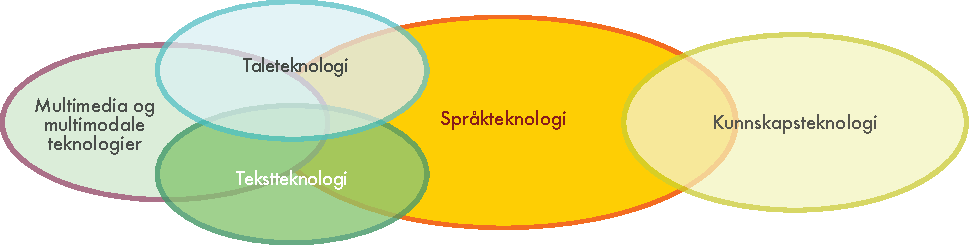
\includegraphics[width=\textwidth]{../_media/norwegian-bokmaal/language_technologies}
  \caption{Språkteknologi}
  \label{fig:ltincontext_no}
  \colorrule{grey3}{\textwidth}{1.5pt}
\end{figure*}

Når vi kommuniserer, kombinerer vi språk med andre kommunikasjonsmåter og informasjonsmedia -- for eksempel kan det å snakke omfatte både gester og ansiktsuttrykk. Digitale tekster kan knytte seg opp mot både bilder og lyd. Filmer kan inneholde språk i både muntlig og skriftlig form. Med andre ord er tale- og tekst-teknologi overlappende, og de samhandler med andre teknologiske verktøy som bidrar til behandling av multimodal kommunikasjon og multimediadokumenter.\\ 
I det følgende vil vi diskutere de viktigste bruksområdene for språkteknologi, nemlig korrekturlesning, nettsøk, taleteknologi og maskinoversettelse. 

Dette omfatter programmer og grunnleggende teknologier som:

\begin{itemize}
\item korrekturlesning
\item skrivestøtte
\item data-assistert språklæring
\item informasjonsinnhenting  
\item informasjonsekstrahering
\item tekstsammendrag
\item besvarelse av spørsmål/dialogsystemer
\item talegjenkjenning 
\item talesyntese 
\end{itemize}

Språkteknologi er et etablert forskningsfelt, og det finnes et omfattende utvalg av introduksjonslitteratur.

%start Norwegian
For videre lesning anbefales lærebøkene \cite{jurafsky-martin01, manning-schuetze1}, oversiktsverkene \cite{lt-survey1} og nettsiden LT World (\url{http://www.lt-world.org}).
%end Norwegian

Før vi går videre til en diskusjon av disse bruksområdene, skal vi kort beskrive oppbyggingen av et typisk språkteknologisk system.

\subsection[Applikasjonsarkitekturer]{Applikasjons- arkitekturer}

Dataprogrammer for språkbehandling består typisk av flere komponenter som gjenspeiler ulike aspekter ved språket. Slike applikasjoner er som oftest svært komplekse, og figur~\ref{fig:textprocessingarch_no} viser en svært forenklet arkitektur for et vanlig tekstbehandlingsprogram. De tre første modulene håndterer strukturen og betydningen til den analyserte teksten:

\begin{enumerate}
\item Preprosessering: Renser data, analyserer eller fjerner formattering, identifiserer  inndataspråk, osv.
\item Grammatisk analyse: Finner verbet, identifiserer verbets objekter, modifikatorer og andre setningskomponenter, identifiserer setningsstruktur.
\item Semantisk analyse: Utfører disambiguering (dvs. beregner betydningen av et ord i en gitt kontekst); løser opp anaforer (dvs. finner hvilket pronomen som refererer til hvilket substantiv i setningen); representerer setningens betydning på en maskinlesbar måte.
\end{enumerate}

Etter tekstanalysen kan moduler innrettet mot spesifikke oppgaver tas i bruk, for eksempel automatisk sammendrag og databasesøk. 

I resten av dette kapittelet skal vi først gi en beskrivelse av de viktigste bruksområdene for språkteknologi. Deretter følger en kort oversikt over situasjonen for språkteknologisk forskning og utdanning i dag, sammen med en beskrivelse av tidligere og nåværende forskningsprogrammer. Til slutt presenteres et ekspertestimat for de viktigste språkteknologiske verktøyene og ressursene for norsk, vurdert etter ulike kriterier som tilgjengelighet, modenhetsnivå og kvalitet. Den generelle situasjonen for språkteknologi for norsk språk er oppsummert i en egen tabell (figur~\ref{fig:lrlttable_no}, s.~\pageref{fig:lrlttable_no}), som gir en oppdatert oversikt over språkteknologi for norsk. Den språkteknologiske støtten for norsk språk er også sammenliknet med de andre språkene som er analysert i denne hvitbokserien.

\begin{figure*}[htb]
  \colorrule{grey3}{\textwidth}{1.5pt}
  \center
  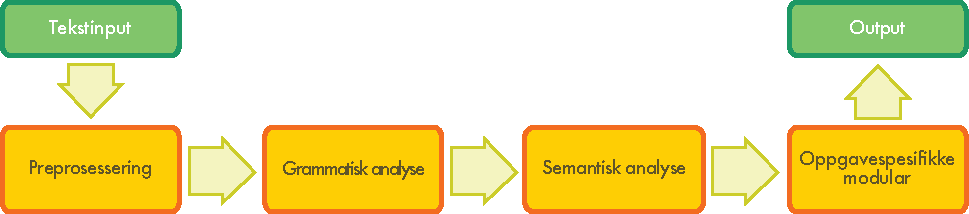
\includegraphics[width=\textwidth]{../_media/norwegian-bokmaal/text_processing_app_architecture}
  \caption{En typisk applikasjonsarkitektur for tekstprosessering}
  \label{fig:textprocessingarch_no}
  \colorrule{grey3}{\textwidth}{1.5pt}
\end{figure*}

\subsection{De viktigste bruksområdene}

I dette delkapittelet fokuserer vi på de viktigste språkteknologiske verktøyene og ressursene, og gir en oversikt over språkteknologisk virksomhet i Norge. 

\subsubsection{Korrekturlesningsverktøy}

Alle som har brukt et tekstbehandlingsprogram som Microsoft Word vet at den har en stavekontroll som uthever stavefeil og foreslår rettelser. De første stavekontrollene  sammenlignet en liste av utvalgte ord mot en ordbok med korrekte ord. I dag er slike programmer langt mer sofistikerte. Ved å bruke språkspesifikke algoritmer for \textbf{grammatisk analyse} kan de oppdage morfologiske feil (f.\,eks.~flertallsformer) samt syntaktiske feil, som manglende verb eller gal verbbøyning (f.eks \textit{hun *skrive et brev}). Men de fleste korrekturverktøyene vil ikke finne noen feil i følgende engelske tekst, fordi alle ordene er korrekt stavet, selv om noen av ordvalgene faktisk er feil \cite{zar1}:
 
\begin{quote}
  I have a spelling checker,\\
  It came with my PC.\\
  It plane lee marks four my revue\\
  Miss steaks aye can knot sea.
\end{quote}

%start Norwegian
For å avdekke slike feil trengs en analyse av konteksten, for eksempel for å avgjøre om et norsk ord skal staves med enkel eller dobbel konsonant i norsk, som i \textit{vil} vs. \textit{vill}.
Denne typen analyse må enten baseres på språkspesifikke \textbf{grammatikker} som eksperter møysommelig har kodet i programvaren, eller på en statistisk språkmodell. 
I en statistisk modell beregnes da sannsynligheten for at et bestemt ord forekommer i en bestemt posisjon i teksten. For eksempel er \textit{jeg vil ha} en mye mer sannsynlig ordsekvens enn \textit{jeg vill ha}. En statistisk språkmodell kan genereres automatisk ved hjelp av en stor mengde av (riktige) språkdata, et \textbf{tekstkorpus}. 

Disse to tilnærmingene har i hovedsak blitt utviklet med utgangspunkt i materiale fra engelsk. Imidlertid kan ingen av dem enkelt overføres til norsk, siden norsk har annerledes ordstilling, sammensatte ord og et mer omfattende bøyningsmønster for visse ordklasser enn engelsk. Studier med utgangspunkt i norsk er derfor nødvendig. Siden norsk har to offisielle målformer, hvorav den ene er mindre brukt, er behovet for gode korrekturverktøy for hver av målformene betydelig.

\begin{figure*}[htb]
  \colorrule{grey3}{\textwidth}{1.5pt}
  \center
  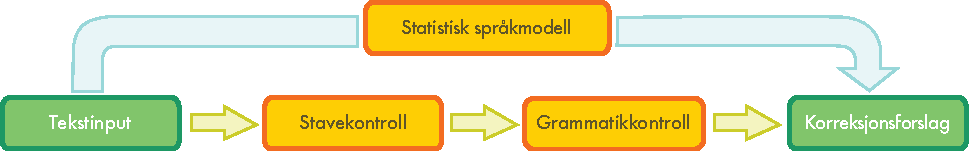
\includegraphics[width=\textwidth]{../_media/norwegian-bokmaal/language_checking}
  \caption{Korrekturlesning (over: statistisk; under: regelbasert)}
  \label{fig:langcheckingaarch_no}
  \colorrule{grey3}{\textwidth}{1.5pt}
\end{figure*}

Korrekturlesningsverktøy er ikke begrenset til tekstbehandlingsprogrammer, det er også brukt i  “skrivestøttesystemer”, dvs. programvaresystemer som brukes for å skrive manualer og andre typer teknisk dokumentasjon som må oppfylle spesielle standarder for eksempel innen IT- og helsesektoren og innen ingeniørvirksomhet. I frykt for kundeklager og skadekrav som følge av uklare instruksjoner, fokuserer næringslivet i økende grad på teknisk dokumentasjonskvalitet, samtidig som de retter seg mot et internasjonalt marked (via oversettelses- eller lokaliseringstjenester). Fremskritt innen prosessering av naturlig språk har ført til utvikling av programvare for skrivestøtte. Slik programvare hjelper forfattere av teknisk dokumentasjon til å bruke ordforråd og setningsstrukturer som er i samsvar med industriregler og (bedriftsinterne) terminologiske restriksjoner.

\boxtext{Korrekturlesningsverktøy brukes ikke bare til tekstbehandling, det brukes også i skrivestøttesystemer.}

%start Norwegian
Gode korrekturlesningsverktøy kan være et viktig redskap for personer med skrivevansker, det være seg dyslektikere eller andrespråkselever, siden en kontekstsensitiv analyse gjør det mulig å foreslå færre og mer relevante stavemåter; det motsatte, mange valg, krever nettopp et høyt nivå av leseferdighet og språklig bevissthet.

Enkelte norske selskaper og språktjenesteleverandører utvikler produkter på dette området. 
I forskningssektoren utvikles grunnleggende språkteknologiske ressurser som kan være av nytte for grammatikk- og stavekontroll (leksikon, ordlister, tekstkorpus, analyseverktøy for sammensatte ord); disse er i hovedsak utviklet ved Universitetet i Oslo, Universitetet i Bergen og Uni Research i Bergen.

Det mest brukte korrekturverktøyet for norsk finnes i Microsoft Office-pakken, og er laget av det finske firmaet Lingsoft, mens deler av grammatikkontrollen for bokmål ble utviklet av forskere ved Universitetet i Oslo. Stavekontroll for bokmål og nynorsk med åpen kilde-teknologi, som \textit{Hunspell}, er også tilgjengelig. 

En annen norsk kommersiell aktør er Tansa, som spesialiserer seg på korrekturverktøy tilpasset større bedrifters spesifikke behov og ordforråd. 
De dekker flere språk i tillegg til norsk bokmål og nynorsk (for eksempel engelsk, tysk, spansk og fransk), og kundene spenner fra NRK til Financial Times. 
Nynodata AS tilbyr et oversettelsesverktøy fra bokmål til nynorsk som samtidig hjelper brukeren å følge en konsekvent formbruk.

Tre selskaper retter seg spesifikt mot skriftlige hjelpemidler for dyslektikere. To av dem, Lingit og Include, inneholder en stavekontrollmodul i tillegg til andre lese- og skriveverktøy (ordprediksjon, tekst-til-tale-komponenter), mens MikroVerkstedet tilbyr fullføring av ord og ordprediksjon.

Ved første øyekast fremstår dermed situasjonen for korrekturverktøy på norsk som god. 
Men samtidig er flere av initiativene nokså sårbare. 
For eksempel er norsk korrekturlesning basert på åpen kildekode (\textit{aspell, Hunspell}) drevet av tre enkeltpersoner som gjør dette på fritiden. 
Med andre ord er en av de viktigste norske konkurrentene til Microsofts programvare avhengig av et personlig initiativ fra en håndfull idealistiske enkeltpersoner, snarere enn en systematisk innsats for å utvikle moduler med åpen kildekode. 
Videre er det en viktig utfordring for de fleste norske korrekturlesningsverktøyene å \textit{forbedre} eksisterende ressurser ved å utvikle mer avanserte språkteknologiske verktøy.  Det mangler også språkspesifikke verktøy for automatisk oversettelse og oversettelsesstøtte. Verktøy med oversettelsesminne som Trados finnes, men de har ingen språkspesifikk tilpasning til norsk utover en grunnleggende stavekontroll.

Utover korrekturlesning og skrivestøtte er korrekturverktøy også viktig innenfor data-assistert språklæring. Korrekturverktøy kan også automatisk korrigere nettsøk, som i Googles \textit{Mente du…}  - forslag til korrekte nettsøk.
%end Norwegian

\subsubsection{Nettsøk}

\begin{figure*}[htb]
  \colorrule{grey3}{\textwidth}{1.5pt}
  \center
  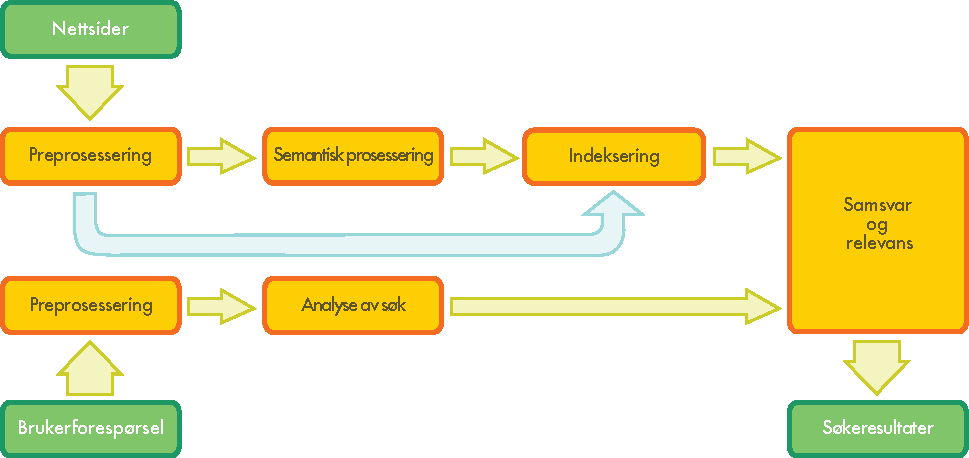
\includegraphics[width=\textwidth]{../_media/norwegian-bokmaal/web_search_architecture}
  \caption{Nettsøk}
  \label{fig:websearcharch_no}
  \colorrule{grey3}{\textwidth}{1.5pt}
 \end{figure*}

Digitale søk er sannsynligvis den mest brukte språkteknologiske applikasjonen, men den er samtidig i stor grad underutviklet. Søkemotoren Google, som ble opprettet i 1998, utfører nå omtrent 80\% av alle nettsøk \cite{spi1}. 
Googles søkegrensesnitt og resultatvisning har ikke endret seg vesentlig siden den første versjonen. Men i den nåværende versjonen tilbyr Google stavekorrigering for feilstavede ord, og har innarbeidet grunnleggende semantiske søkemuligheter som kan forbedre nøyaktigheten gjennom analyser av ordets betydning i en gitt søkekontekst \cite{pc1}. Googles suksess viser at med store mengder tilgjengelige data kan statistiske metoder gi relativt gode resultater.

For mer sofistikerte informasjonssøk er det imidlertid avgjørende å integrere dypere lingvistiske analyser for teksttolkning. Eksperimenter med \textbf{leksikalske ressurser}, som maskinlesbare tesauruser eller ontologiske språkressurser (for eksempel WordNet for engelsk; et norsk ordnett er ventet innen utgangen av 2012), har gitt bedre resultater når det gjelder å finne nettsider som inneholder synonymer til den opprinnelige søketermen, som 
\textit{atomkraft}, \textit{kjerneenergi} og \textit{nukleærenergi}, og til og med termer som er enda løsere beslektet.  

\boxtext{Den neste generasjonen søkemotorer må bruke en mye mer sofistikert språkteknologi.}

Den neste generasjonen søkemotorer må bruke en mye mer sofistikert språkteknologi, særlig for søk som består av et spørsmål eller en annen type setning, og ikke bare en liste av nøkkelord. For å svare på søket \textit{Gi meg en liste over alle selskaper som har blitt tatt over av et annet selskap de siste fem årene}, må systemet gjøre en \textbf{syntaktisk} og \textbf{semantisk analyse} av setningen og lage en hurtig oversikt over relevante dokumenter. Et tilfredsstillende svar forutsetter en syntaktisk analyse av setningens grammatiske struktur for å slå fast at brukeren spør etter selskaper som har blitt kjøpt opp, ikke selskaper som har kjøpt opp andre. Når det gjelder uttrykket \textit{de siste fem årene} må systemet avgjøre hvilke år det dreier seg om. Søket må så sammenlignes mot en stor mengde ustrukturerte data for å finne relevante treff. Dette kalles informasjonshenting (engelsk \textit{Information Retrieval}), og omfatter søk og rangering av relevante dokumenter. For å lage en liste over selskapene trenger systemet også å forstå at en bestemt ordstreng i et dokument er navnet på et selskap, en prosess som kalles navnegjenkjenning.

En enda større utfordring er å forsøke å finne treff på et søk i dokumenter på et annet språk. Ved informasjonssøk på tvers av språk må søkeordet oversettes automatisk til alle potensielle kildespråk, og resultatene må i sin tur oversettes tilbake til brukerens språk.   

Siden data i økende grad oppbevares i andre formater enn tekst, trengs en tjeneste for multimedial informasjonsinnhenting som lar oss søke i bilder, lydfiler og videomateriale. Når det gjelder lyd- og videofiler må en talegjenkjenningsmodul konvertere taleinnholdet til tekst (eller fonetiske representasjoner) som så kan gi treff mot et brukersøk.

I Norge utviklet Opera Software den første norske nettleseren og Internettprogramvaren. Opera begynte i 1994 som et forskningsprosjekt i Telenor. 
Etter et år ble det skilt ut som et uavhengig utviklingsselskap, Opera Software ASA. Enkelte norske selskaper utvikler eller appliserer søkeløsninger (CognIT, Comperio, TextUrgy, Abtrox og  Infofinder). 
FAST utviklet en søkemotor som ble kjøpt opp av Microsoft, og som nå forhandles av Comperio. 
Utviklingsfokuset til disse selskapene er generelt rettet mot å tilby tilleggsprogrammer og avanserte søkemotorer som utnytter domenerelevant informasjon.
IT-industrien i Norge har altså allerede et ganske godt grunnlag når det gjelder nettsøk og informasjonsinnhenting; det største behovet som bedriftene rapporterer om gjelder kvalitetssikrede språkteknologiske komponenter.
%end Norwegian

\subsubsection{Taleteknologi}

De grunnleggende taleteknologiene er talegjenkjenning og talesyntese, som kan brukes til å utvikle talebasert interaksjon og dialogsystemer. Taleteknologi brukes for å lage grensesnitt som lar brukerne samhandle gjennom talespråk heller enn å bruke en grafisk skjerm, tastatur og mus. I dag brukes talegrensesnitt til helt og delvis automatiserte telefontjenester som selskaper tilbyr sine kunder, ansatte eller partnere. Talegrensesnitt brukes i stor grad til blant annet banktjenester, distribusjonskjeder, kollektivtransport og i telesektoren. Taleteknologi brukes også til grensesnitt for navigasjonssystemer i biler og til bruk av talespråk som et alternativ til grafiske grensesnitt eller trykkfølsomme skjermer i smarttelefoner.  

\begin{figure*}[htb]
  \colorrule{grey3}{\textwidth}{1.5pt}
  \center
  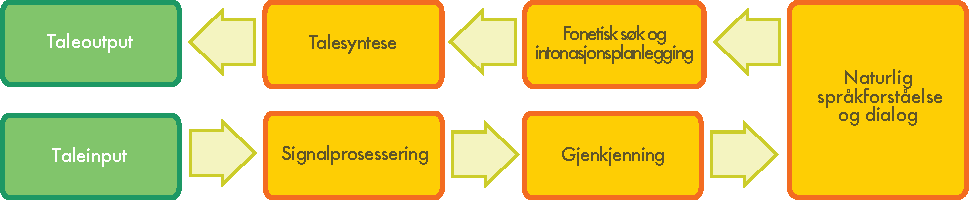
\includegraphics[width=\textwidth]{../_media/norwegian-bokmaal/simple_speech-based_dialogue_architecture}
  \caption{Talebasert dialogsystem}
  \label{fig:dialoguearch_no}
  \colorrule{grey3}{\textwidth}{1.5pt}
\end{figure*}

Taleteknologi omfatter fire typer verktøy: 

\begin{enumerate}
\item Automatisk \textbf{talegjenkjenning} (tale-til-tekst) avgjør hvilke ord som faktisk sies i en gitt lydsekvens ytret av en språkbruker.
\item Naturlig språkforståelse analyserer ytringens syntaktiske struktur, og tolker den ut fra systemet som brukes. 
\item Dialogstyring avgjør hvilken handling som skal utføres, gitt et bestemt brukerinput og en viss systemfunksjonalitet.
\item \textbf{Talesyntese} (tekst-til-tale) omskaper systemets svar til lyder som er forståelige for brukeren.
\end{enumerate}

Automatiske talegjenkjenningssystemer forsøker å gjenkjenne ordene som ytres. Det betyr at utvalget av mulige ytringer må avgrenses til et begrenset sett av nøkkelord, eller at man manuelt lager språkmodeller som dekker et stort omfang av naturlige språkytringer. Ved hjelp av maskinlæringsteknikker kan man også automatisk generere språkmodeller fra \textbf{talekorpus}, dvs. store samlinger av tale i lydfiler og teksttranskripsjoner. Å begrense ytringene innebærer vanligvis at brukerne pålegges å bruke grensesnittet på en begrenset måte, hvilket kan svekke brukerens aksept av verktøyet. På den annen side vil det øke kostnadene betraktelig å skape, fininnstille og vedlikeholde rike språkmodeller. Talegrensesnitt som bruker språkmodeller og lar brukeren uttrykke seg mer fleksibelt i begynnelsen – ved hjelp av et spørsmål som: \textit{Hva kan jeg gjøre for deg?} – er generelt automatisert, og gir ofte en bedre opplevelse for brukerne. 

\boxtext{Taleteknologi brukes for å lage grensesnitt som lar brukerne samhandle gjennom talespråk heller enn å bruke en grafisk skjerm, tastatur og mus.}

Bedrifter bruker ofte forhåndsinnspilt tale, innspilt av  profesjonelle, for å generere materialet som skal brukes i talegrensesnitt. For statiske ytringer, hvor formuleringene ikke avhenger av en bestemt situasjon eller personlige brukerdata, kan dette gi en god brukeropplevelse. Men mer dynamisk ytringsinnhold kan preges av unaturlig intonasjonsmønstre, fordi de rett og slett produseres ved å lime ulike lydfiler sammen. Dagens talesyntese er blitt stadig bedre til å produsere dynamiske ytringer som høres naturlige ut, selv om de fremdeles har et forbedringspotensial. 

Det siste tiåret har det skjedd en betydelig standardisering av talegrensesnitt når det gjelder de ulike teknologiske komponentene. Det har  også vært en sterk markedskonsolidering innen taleteknologi. I G20-landene (de 19 landene i verden med best økonomi samt EU) har kun fem globale aktører dominert markedet, med Nuance (USA) og Loquendo (Italia) som de viktigste i Europa. I 2011 kunngjorde Nuance oppkjøpet av Loquendo, og dette innebar et nytt steg i retning av en sterkere konsolidering av markedet. 

%start Norwegian
For norsk talesyntese finnes tretten norske stemmer; de fleste har blitt utviklet av aktørene vi har nevnt ovenfor. 
Tre av stemmene er utviklet av den norske bedriften Lingit, som retter seg mot brukere med lese- og skrivevansker. 
En annen stemme ble utviklet ved Norsk lyd- og blindeskriftbibliotek i samarbeid med søsterbiblioteket i Sverige. 
Der er også en aktiv forskergruppe ved NTNU i Trondheim.

\boxtext{Språkressurser for talesyntese finnes på engelsk, men bare i liten grad for norsk.}

Kvaliteten på talesyntese er sterkt avhengig av tilgjengelige resursser (spesielt tekstkorpus tagget med informasjon om ordklasse, tokenisatorer og uttaleleksika) og språkspesifikk forskning på for eksempel prosodiske trekk i det aktuelle språket. 
Det finnes mange slike ressurser på engelsk, men bare i liten grad for norsk. Likevel er behovet ekstra stort for norsk på grunn av det store mangfoldet i mulige stavemåter og dialekter, i tillegg til utfordringer knyttet til tonelag og en manglende én-til-én-relasjon mellom lyder og bokstaver.

Når det gjelder teknologi og kunnskap for dialogstyring er det norske markedet dominert av mindre, norske bedrifter. 
MediaLT har utviklet en generell talegjenkjenner som brukes til dialogstyring for blinde og svaksynte. 
Innen tale-til-tekst har Max Manus integrert og tilrettelagt Phillips’ SpeechMagic for norske sykehus. 
Systemet er relativt vellykket, men har et relativt avgrenset bruksområde med et lukket vokabular. 
Nylig ble Dragon Dictation, en stemmegjenkjenningsapplikasjon for mobiltelefoner, lansert for norsk. 
Denne applikasjonen er det første \textit{generelle} dikteringssystemet for norsk, men den norske versjonen av Dragon Dictation later til å gi betydelig mer feiltolking enn den engelske versjonen.
For taleinteraksjon finnes det ennå ikke et fungerende marked for lingvistiske kjerneteknologier for syntaktisk og semantisk analyse.
%end Norwegian

I tiden fremover kan man sannsynligvis vente en betydelig utvikling på grunn av økt bruk av smarttelefoner som en ny plattform for å håndtere kunderelasjoner, i tillegg til allerede eksisterende kommunikasjonsmedia som fasttelefoner, Internett og e-post.
Dette vil sannsynligvis også påvirke bruken av taleteknologi og dialogsystemer. På sikt vil der sannsynligvis bli færre telefonbaserte talegrensesnitt, og talespråksapplikasjoner vil spille en langt mer sentral rolle som en brukervennlig interasjonsmåte med smarttelefoner.
Denne utviklingen vil sannsynligvis primært drives frem gjennom stegvise forbedringer av talegjenkjenningssystemer som ikke er fokusert på én bestemt bruker, via dikteringssystemer som allerede tilbys som sentraliserte tjenester for smarttelefonbrukere.

\subsubsection{Maskinoversettelse}

\begin{figure*}[htb]
  \colorrule{grey3}{\textwidth}{1.5pt}
  \center
  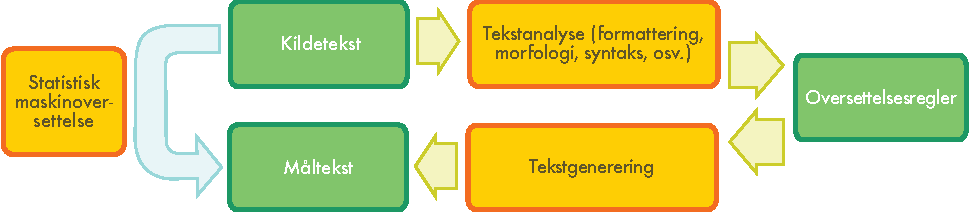
\includegraphics[width=\textwidth]{../_media/norwegian-bokmaal/machine_translation}
  \caption{Maskinoversettelse (venstre: statistisk; høyre: regelbasert)}
  \label{fig:mtarch_no}
  \colorrule{grey3}{\textwidth}{1.5pt}
\end{figure*}

Tanken om å bruke datamaskiner til å oversette naturlig språk ble introdusert i 1946, og utløste en omfattende forskningsinnsats på 50-tallet, som så ble gjenopplivet på 80-tallet. Likevel har \textbf{maskinoversettelse} (MO) fremdeles ikke levd opp til de tidlige forhåpningene om å kunne tilby generell, automatisert oversettelse.

\boxtext{Maskinoversettelse er først og fremst vanskelig fordi menneskelig språk er flertydig.}

Den mest grunnleggende tilnærmingen til maskinoversettelse er automatisk å erstatte ord i et språk med ord i et annet språk. Dette kan fungere bra for domener hvor ordforrådet er begrenset og standardisert, som for eksempel værmeldinger. Men for å lage gode oversettelser av tekster fra mer generelle domener må man oversette større tekstbiter (ordgrupper, setninger, eller til og med hele avsnitt), og hver tekstbit må stemme overens med tilsvarende del i kildeteksten. Maskinoversettelse er først og fremst vanskelig fordi menneskelig språk er flertydig. 

%start Norwegian
Flertydighet gir utfordringer på flere nivåer, blant annet kan man trenge å løse flertydigheter både på ordnivå og på setningsnivå. 
In en enkel ord-for-ord-oversettelse til engelsk kan setningen \textit{Plutselig røk slangen} derfor gi resultatet \textit{Suddenly smoked the snake.}
Verbformen \textit{røk} (preteritum av \textit{ryke}) er flertydig mellom det vi på engelsk ville oversette som henholdsvis \textit{snap} og \textit{smoke}.
Ordet \textit{slange} er på sin side flertydig mellom `vannslange' (engelsk \textit{hose}) og `reptilslange' (engelsk \textit{snake}). Legg også merke til at en enkel ord-for-ord-oversettelse ikke ville gitt riktig rekkefølge av ordene på engelsk.

I tillegg til leksikalsk flertydighet og forskjeller i ordstilling kommer utfordringer med syntaktiske flertydigheter. På norsk kan man for eksempel topikalisere objektet i en setning, mens mulighetene for å gjøre dette på engelsk er mye mer begrenset. Den norske setningen \textit{Eplene spiste mannen} har to ulike tolkninger: Enten analyseres \textit{eplene} som setningens subjekt (mannen ble spist av eplene), eller som et topikalisert objekt (eplene ble spist av mannen). Siden denne flertydigheten ikke finnes på engelsk, må et maskinoversettelsessystem først finne den korrekte syntaktiske tolkningen for å komme frem til en korrekt oversettelse.

En annen utfordring for maskinoversettelse for norsk er sammensatte ord. Et effektivt oversettelsessystem må kunne identifisere sammensatte ord som ikke står i ordboken, analysere dem, og om nødvendig lage nye sammensatte ord i målspråket.
%end Norwegian

For oversettelser mellom nært beslektede språk kan en enkel ord-for-ord-oversettelse la seg gjøre. Men maskinoversettelsessystemer kan også bygges ved å bruke lingvistiske regler. Regelbaserte (eller kunnskapsdrevne) systemer analyserer kildeteksten, og lager en mellomstående symbolsk representasjon. På grunnlag av den symbolske representasjonen kan man så generere tekst til målspråket. Kvaliteten på slike metoder avhenger i stor grad av tilgangen til omfattende ordbøker med morfologisk, syntaktisk og semantisk informasjon, i tillegg til store sett med grammatiske regler utviklet av  språkforskere. Dette er en veldig omfattende, og derfor dyr, prosess.

På slutten av 80-tallet, da datamaskinkapasiteten økte, økte også interessen for statistiske modeller for maskinoversettelse. Statistiske modeller for maskinoversettelse er basert på analyser av tospråklige tekstkorpus, som \textbf{parallellkorpuset} Europarl, som består av møtereferater fra Europaparlamentet på 21 europeiske språk 
%start Norwegian
(norsk er ikke inkludert).
%end Norwegian
Hvis man har tilgang til tilstrekkelige mengder data, kan statistisk maskinoversettelse fungere godt nok til å utlede den omtrentlige betydningen til en tekst på et annet språk, gjennom å prosessere parallelle versjoner av tekst og dermed finne sannsynlige ordmønstre. Datadrevet maskinoversettelse har sine fordeler, fordi den krever mindre menneskelig innsats, og den kan fange opp særegenheter ved språket (for eksempel idiomatiske uttrykk) som kan bli oversett av kunskapsdrevne systemer. Men i motsetning til kunnskapsdrevne systemer gir statistisk (eller datadrevet) maskinoversettelse ofte ugrammatiske resultater.  

Ofte er det altså slik at fordelene og ulempene ved kunnskapsdrevet og datadrevet maskinoversettelse utfyller hverandre. Derfor fokuserer nyere forskning ofte på hybridtilnærminger som kombinerer begge metodene. Én slik tilnærming bruker både kunnskapsdrevne og datadrevne systemer sammen med en selekteringsmodul som avgjør det beste resultatet for hver setning. For setninger lengre enn omtrent tolv ord blir imidlertid resultatene som regel mindre gode. Her kan en bedre løsning være å kombinere de beste delene fra hver setning fra flere ulike kilder. Dette kan være en ganske kompleks oppgave, siden siden det ikke alltid er klart hvilke av flere ulike muligheter som passer sammen. Disse må identifiseres og parallellstilles.   

%start Norwegian

Når det gjelder oversettelse mellom de to norske målformene er behovet for effektive oversettelsesverktøy stort. To selskaper har utviklet systemer for dette; Nynodata og Apertium. Nynodata er en liten bedrift som tilbyr verktøy for oversettelse, korrektur og tekstsøk for bokmål og nynorsk. Apertium er et åpen-kilde-initiativ som også tilbyr automatisert oversettelse mellom de to målformene, implementert av en student ved Universitetet i Bergen.

\boxtext{Selv om det er et klart behov for maskinoversettelse for norsk, er utviklingen av slik programvare for norsk ennå ikke omfattende.}

Når det gjelder oversettelse mellom norsk og ulike fremmedspråk har Google Translate en norsk modul for oversettelse mellom engelsk og norsk; via engelsk er det mulig å oversette mellom norsk og ethvert språkpar som inneholder engelsk. GramTrans er en maskinoversettelsesplattform som er utviklet av det danske GrammarSoft ApS og den norske bedriften Kaldera Språkteknologi AS. Denne oversettelsesmotoren tilbyr en tjeneste for gratis, nettbasert oversettelse for de skandinaviske språkene og mellom norsk og engelsk. Programmet er basert på en robust grammatikkanalyse, en transferkomponent som behandler overgangen fra et språk til et annet med hensyn til leksikon og grammatikk, og til slutt en komponent som genererer oversatt tekst på målspråket. Selskapet Clue Norge spesialiserer seg på elektroniske ordbøker for næringslivet, og utviklet for omtrent ti år siden systemet Textran for maskinoversettelse fra engelsk til norsk. Systemet eksisterer fortsatt, men har ikke blitt videreutviklet fordi jevnt pålitelige maskinoversettelser av høy kvalitet er meget vanskelig å oppnå, mens brukergruppene ikke ønsket å betale for et system som gjorde feil. Selv om det foregår en betydelig forskningsinnsats på dette området, både nasjonalt og internasjonalt, har datadrevne og hybride systemer så langt vært mindre vellykket i applikasjoner for næringslivet enn i forskningslaboratoriet. I Norge finnes den viktigste forskningsekspertisen ved Universitetet i Oslo og Universitetet i Bergen.

\boxtext{Språktjenesteindustrien i Norge later til å ha et underforbruk av språkteknologiske ressurser.}

Bruk av maskinoversettelse kan øke produktiviteten betydelig, forutsatt at systemet er tilpasset brukerspesifikk terminologi og er godt integrert i arbeidsflyten på en arbeidsplass. Generelt later imidlertid språktjenesteindustrien i Norge til å ha et underforbruk av språkteknologiske ressurser. 
Sektoren kan deles i to grupper: på den ene siden har man frilansoversettere og oversetterbyråer som retter seg mot enkeltpersoner, næringslivet og offentlig sektor; på den andre siden har man oversettere som er tilknyttet Oversetterforeningen og Norsk faglitterær forfatter- og oversetterforening.

I den siste gruppen framstår bruken av språkteknologi som begrenset. Den førstnevnte gruppen bruker ofte Trados, som er det klart mest brukte oversettelsesverktøyet for profesjonelle oversettere. Trados har imidlertid ingen egen modul for norsk, men støtter seg i stedet på Hunspell, en åpen-kilde-løsning med stavekontroll og et morfologisk analyseverktøy som opprinnelig ble utviklet for ungarsk. Selv om det er en funksjonell og åpen løsning, trenger den ytterligere utvikling for å fungere som en optimal ressurs for språktjenestesektoren i Norge. Særlig stort er behovet for å forbedre analysen av sammensatte ord på norsk. I tillegg bruker profesjonelle oversettere termbaser (DU, IATE), og til en viss grad er der et samarbeid med universitetssektoren i utviklingen av termbaser. Det tilsynelatende underforbruket av språkteknologiske ressurser i språktjenesteindustrien skyldes delvis mangelen på gode ressurser for norsk, men også manglende kontakt mellom språktjenesteleverandører og forskermiljøene. Derfor kan kunnskap om det fulle potensialet for språkteknologi blir for begrenset, og det kan være vanskelig for kommersielle aktører å vurdere kvaliteten på eksisterende ressurser.
%end Norwegian

Kvaliteten på maskinoversettelsessystemer har fremdeles et stort forbedringspotensial. Blant utfordringene er å tilpasse språkressurser til et gitt emne eller brukerområde, og å integrere teknologien i en arbeidsflyt som allerede inneholder termbaser og oversettelsesminne. I tillegg er de fleste systemene som er i bruk rettet mot engelsk, og støtter bare sjelden oversettelse til og fra norsk. Dette gir forstyrrelser i prosessen med å få tekst oversatt, og tvinger maskinoversettelsesbrukere til å lære seg ulike kodingsverktøy for forskjellige systemer.

\begin{figure*}[tb]
  \centering
  \setlength{\tabcolsep}{0.17em}
  \small
  \begin{tabular}{>{\columncolor{corange1}}cccccccccccccccccccccccc}
    & \multicolumn{22}{>{\columncolor{corange1}}c}{Målspråk -- \textcolor{grey1}{Target language}}\\\addlinespace[{-.009cm}]
    \rowcolor{corange1}  & EN & BG & DE & CS & DA & EL & ES & ET & FI & FR & HU & IT & LT & LV & MT & NL & PL & PT & RO & SK & SL & SV\\
    EN & -- & \textcolor{blue}{40.5} & \textcolor{blue}{46.8} & \textcolor{green2}{52.6} & \textcolor{green2}{50.0} & \textcolor{blue}{41.0} & \textcolor{green2}{55.2} & \textcolor{purple}{34.8} & \textcolor{purple}{38.6} & \textcolor{green2}{50.1} & \textcolor{purple}{37.2} & \textcolor{green2}{50.4} & \textcolor{purple}{39.6} & \textcolor{blue}{43.4} & \textcolor{purple}{39.8} & \textcolor{green2}{52.3} & \textcolor{blue}{49.2} & \textcolor{green2}{55.0} & \textcolor{blue}{49.0} & \textcolor{blue}{44.7} & \textcolor{green2}{50.7} & \textcolor{green2}{52.0}\\
    BG & \textcolor{green}{61.3} & -- & \textcolor{purple}{38.7} & \textcolor{purple}{39.4} & \textcolor{purple}{39.6} & \textcolor{purple}{34.5} & \textcolor{blue}{46.9} & \textcolor{red3}{25.5} & \textcolor{red3}{26.7} & \textcolor{blue}{42.4} & \textcolor{red3}{22.0} & \textcolor{blue}{43.5} & \textcolor{red3}{29.3} & \textcolor{red3}{29.1} & \textcolor{red3}{25.9} & \textcolor{blue}{44.9} & \textcolor{purple}{35.1} & \textcolor{blue}{45.9} & \textcolor{purple}{36.8} & \textcolor{purple}{34.1} & \textcolor{purple}{34.1} & \textcolor{purple}{39.9}\\
    DE & \textcolor{green2}{53.6} & \textcolor{red3}{26.3} & -- & \textcolor{purple}{35.4} & \textcolor{blue}{43.1} & \textcolor{purple}{32.8} & \textcolor{blue}{47.1} & \textcolor{red3}{26.7} & \textcolor{red3}{29.5} & \textcolor{purple}{39.4} & \textcolor{red3}{27.6} & \textcolor{blue}{42.7} & \textcolor{red3}{27.6} & \textcolor{purple}{30.3} & \textcolor{red2}{19.8} & \textcolor{green2}{50.2} & \textcolor{purple}{30.2} & \textcolor{blue}{44.1} & \textcolor{purple}{30.7} & \textcolor{red3}{29.4} & \textcolor{purple}{31.4} & \textcolor{blue}{41.2}\\
    CS & \textcolor{green2}{58.4} & \textcolor{purple}{32.0} & \textcolor{blue}{42.6} & -- & \textcolor{blue}{43.6} & \textcolor{purple}{34.6} & \textcolor{blue}{48.9} & \textcolor{purple}{30.7} & \textcolor{purple}{30.5} & \textcolor{blue}{41.6} & \textcolor{red3}{27.4} & \textcolor{blue}{44.3} & \textcolor{purple}{34.5} & \textcolor{purple}{35.8} & \textcolor{red3}{26.3} & \textcolor{blue}{46.5} & \textcolor{purple}{39.2} & \textcolor{blue}{45.7} & \textcolor{purple}{36.5} & \textcolor{blue}{43.6} & \textcolor{blue}{41.3} & \textcolor{blue}{42.9}\\
    DA & \textcolor{green2}{57.6} & \textcolor{red3}{28.7} & \textcolor{blue}{44.1} & \textcolor{purple}{35.7} & -- & \textcolor{purple}{34.3} & \textcolor{blue}{47.5} & \textcolor{red3}{27.8} & \textcolor{purple}{31.6} & \textcolor{blue}{41.3} & \textcolor{red3}{24.2} & \textcolor{blue}{43.8} & \textcolor{red3}{29.7} & \textcolor{purple}{32.9} & \textcolor{red3}{21.1} & \textcolor{blue}{48.5} & \textcolor{purple}{34.3} & \textcolor{blue}{45.4} & \textcolor{purple}{33.9} & \textcolor{purple}{33.0} & \textcolor{purple}{36.2} & \textcolor{blue}{47.2}\\
    EL & \textcolor{green2}{59.5} & \textcolor{purple}{32.4} & \textcolor{blue}{43.1} & \textcolor{purple}{37.7} & \textcolor{blue}{44.5} & -- & \textcolor{green2}{54.0} & \textcolor{red3}{26.5} & \textcolor{red3}{29.0} & \textcolor{blue}{48.3} & \textcolor{red3}{23.7} & \textcolor{blue}{49.6} & \textcolor{red3}{29.0} & \textcolor{purple}{32.6} & \textcolor{red3}{23.8} & \textcolor{blue}{48.9} & \textcolor{purple}{34.2} & \textcolor{green2}{52.5} & \textcolor{purple}{37.2} & \textcolor{purple}{33.1} & \textcolor{purple}{36.3} & \textcolor{blue}{43.3}\\
    ES & \textcolor{green}{60.0} & \textcolor{purple}{31.1} & \textcolor{blue}{42.7} & \textcolor{purple}{37.5} & \textcolor{blue}{44.4} & \textcolor{purple}{39.4} & -- & \textcolor{red3}{25.4} & \textcolor{red3}{28.5} & \textcolor{green2}{51.3} & \textcolor{red3}{24.0} & \textcolor{green2}{51.7} & \textcolor{red3}{26.8} & \textcolor{purple}{30.5} & \textcolor{red3}{24.6} & \textcolor{blue}{48.8} & \textcolor{purple}{33.9} & \textcolor{green2}{57.3} & \textcolor{purple}{38.1} & \textcolor{purple}{31.7} & \textcolor{purple}{33.9} & \textcolor{blue}{43.7}\\
    ET & \textcolor{green2}{52.0} & \textcolor{red3}{24.6} & \textcolor{purple}{37.3} & \textcolor{purple}{35.2} & \textcolor{purple}{37.8} & \textcolor{red3}{28.2} & \textcolor{blue}{40.4} & -- & \textcolor{purple}{37.7} & \textcolor{purple}{33.4} & \textcolor{purple}{30.9} & \textcolor{purple}{37.0} & \textcolor{purple}{35.0} & \textcolor{purple}{36.9} & \textcolor{red3}{20.5} & \textcolor{blue}{41.3} & \textcolor{purple}{32.0} & \textcolor{purple}{37.8} & \textcolor{red3}{28.0} & \textcolor{purple}{30.6} & \textcolor{purple}{32.9} & \textcolor{purple}{37.3}\\
    FI & \textcolor{blue}{49.3} & \textcolor{red3}{23.2} & \textcolor{purple}{36.0} & \textcolor{purple}{32.0} & \textcolor{purple}{37.9} & \textcolor{red3}{27.2} & \textcolor{purple}{39.7} & \textcolor{purple}{34.9} & -- & \textcolor{red3}{29.5} & \textcolor{red3}{27.2} & \textcolor{purple}{36.6} & \textcolor{purple}{30.5} & \textcolor{purple}{32.5} & \textcolor{red2}{19.4} & \textcolor{blue}{40.6} & \textcolor{red3}{28.8} & \textcolor{purple}{37.5} & \textcolor{red3}{26.5} & \textcolor{red3}{27.3} & \textcolor{red3}{28.2} & \textcolor{purple}{37.6}\\
    FR & \textcolor{green}{64.0} & \textcolor{purple}{34.5} & \textcolor{blue}{45.1} & \textcolor{purple}{39.5} & \textcolor{blue}{47.4} & \textcolor{blue}{42.8} & \textcolor{green}{60.9} & \textcolor{red3}{26.7} & \textcolor{purple}{30.0} & -- & \textcolor{red3}{25.5} & \textcolor{green2}{56.1} & \textcolor{red3}{28.3} & \textcolor{purple}{31.9} & \textcolor{red3}{25.3} & \textcolor{green2}{51.6} & \textcolor{purple}{35.7} & \textcolor{green}{61.0} & \textcolor{blue}{43.8} & \textcolor{purple}{33.1} & \textcolor{purple}{35.6} & \textcolor{blue}{45.8}\\
    HU & \textcolor{blue}{48.0} & \textcolor{red3}{24.7} & \textcolor{purple}{34.3} & \textcolor{purple}{30.0} & \textcolor{purple}{33.0} & \textcolor{red3}{25.5} & \textcolor{purple}{34.1} & \textcolor{red3}{29.6} & \textcolor{red3}{29.4} & \textcolor{purple}{30.7} & -- & \textcolor{purple}{33.5} & \textcolor{red3}{29.6} & \textcolor{purple}{31.9} & \textcolor{red2}{18.1} & \textcolor{purple}{36.1} & \textcolor{red3}{29.8} & \textcolor{purple}{34.2} & \textcolor{red3}{25.7} & \textcolor{red3}{25.6} & \textcolor{red3}{28.2} & \textcolor{purple}{30.5}\\
    IT & \textcolor{green}{61.0} & \textcolor{purple}{32.1} & \textcolor{blue}{44.3} & \textcolor{purple}{38.9} & \textcolor{blue}{45.8} & \textcolor{blue}{40.6} & \textcolor{red3}{26.9} & \textcolor{red3}{25.0} & \textcolor{red3}{29.7} & \textcolor{green2}{52.7} & \textcolor{red3}{24.2} & -- & \textcolor{red3}{29.4} & \textcolor{purple}{32.6} & \textcolor{red3}{24.6} & \textcolor{green2}{50.5} & \textcolor{purple}{35.2} & \textcolor{green2}{56.5} & \textcolor{purple}{39.3} & \textcolor{purple}{32.5} & \textcolor{purple}{34.7} & \textcolor{blue}{44.3}\\
    LT & \textcolor{green2}{51.8} & \textcolor{red3}{27.6} & \textcolor{purple}{33.9} & \textcolor{purple}{37.0} & \textcolor{purple}{36.8} & \textcolor{red3}{26.5} & \textcolor{red3}{21.1} & \textcolor{purple}{34.2} & \textcolor{purple}{32.0} & \textcolor{purple}{34.4} & \textcolor{red3}{28.5} & \textcolor{purple}{36.8} & -- & \textcolor{blue}{40.1} & \textcolor{red3}{22.2} & \textcolor{purple}{38.1} & \textcolor{purple}{31.6} & \textcolor{purple}{31.6} & \textcolor{red3}{29.3} & \textcolor{purple}{31.8} & \textcolor{purple}{35.3} & \textcolor{purple}{35.3}\\
    LV & \textcolor{green2}{54.0} & \textcolor{red3}{29.1} & \textcolor{purple}{35.0} & \textcolor{purple}{37.8} & \textcolor{purple}{38.5} & \textcolor{red3}{29.7} & \textcolor{red2}{8.0} & \textcolor{purple}{34.2} & \textcolor{purple}{32.4} & \textcolor{purple}{35.6} & \textcolor{red3}{29.3} & \textcolor{purple}{38.9} & \textcolor{purple}{38.4} & -- & \textcolor{red3}{23.3} & \textcolor{blue}{41.5} & \textcolor{purple}{34.4} & \textcolor{purple}{39.6} & \textcolor{purple}{31.0} & \textcolor{purple}{33.3} & \textcolor{purple}{37.1} & \textcolor{purple}{38.0}\\
    MT & \textcolor{green}{72.1} & \textcolor{purple}{32.2} & \textcolor{purple}{37.2} & \textcolor{purple}{37.9} & \textcolor{purple}{38.9} & \textcolor{purple}{33.7} & \textcolor{blue}{48.7} & \textcolor{red3}{26.9} & \textcolor{red3}{25.8} & \textcolor{blue}{42.4} & \textcolor{red3}{22.4} & \textcolor{blue}{43.7} & \textcolor{purple}{30.2} & \textcolor{purple}{33.2} & -- & \textcolor{blue}{44.0} & \textcolor{purple}{37.1} & \textcolor{blue}{45.9} & \textcolor{purple}{38.9} & \textcolor{purple}{35.8} & \textcolor{blue}{40.0} & \textcolor{blue}{41.6}\\
    NL & \textcolor{green2}{56.9} & \textcolor{red3}{29.3} & \textcolor{blue}{46.9} & \textcolor{purple}{37.0} & \textcolor{blue}{45.4} & \textcolor{purple}{35.3} & \textcolor{blue}{49.7} & \textcolor{red3}{27.5} & \textcolor{red3}{29.8} & \textcolor{blue}{43.4} & \textcolor{red3}{25.3} & \textcolor{blue}{44.5} & \textcolor{red3}{28.6} & \textcolor{purple}{31.7} & \textcolor{red3}{22.0} & -- & \textcolor{purple}{32.0} & \textcolor{blue}{47.7} & \textcolor{purple}{33.0} & \textcolor{purple}{30.1} & \textcolor{purple}{34.6} & \textcolor{blue}{43.6}\\
    PL & \textcolor{green}{60.8} & \textcolor{purple}{31.5} & \textcolor{blue}{40.2} & \textcolor{blue}{44.2} & \textcolor{blue}{42.1} & \textcolor{purple}{34.2} & \textcolor{blue}{46.2} & \textcolor{red3}{29.2} & \textcolor{red3}{29.0} & \textcolor{blue}{40.0} & \textcolor{red3}{24.5} & \textcolor{blue}{43.2} & \textcolor{purple}{33.2} & \textcolor{purple}{35.6} & \textcolor{red3}{27.9} & \textcolor{blue}{44.8} & -- & \textcolor{blue}{44.1} & \textcolor{purple}{38.2} & \textcolor{purple}{38.2} & \textcolor{purple}{39.8} & \textcolor{blue}{42.1}\\
    PT & \textcolor{green}{60.7} & \textcolor{purple}{31.4} & \textcolor{blue}{42.9} & \textcolor{purple}{38.4} & \textcolor{blue}{42.8} & \textcolor{blue}{40.2} & \textcolor{green}{60.7} & \textcolor{red3}{26.4} & \textcolor{red3}{29.2} & \textcolor{green2}{53.2} & \textcolor{red3}{23.8} & \textcolor{green2}{52.8} & \textcolor{red3}{28.0} & \textcolor{purple}{31.5} & \textcolor{red3}{24.8} & \textcolor{blue}{49.3} & \textcolor{purple}{34.5} & -- & \textcolor{purple}{39.4} & \textcolor{purple}{32.1} & \textcolor{purple}{34.4} & \textcolor{blue}{43.9}\\
    RO & \textcolor{green}{60.8} & \textcolor{purple}{33.1} & \textcolor{purple}{38.5} & \textcolor{purple}{37.8} & \textcolor{blue}{40.3} & \textcolor{purple}{35.6} & \textcolor{green2}{50.4} & \textcolor{red3}{24.6} & \textcolor{red3}{26.2} & \textcolor{blue}{46.5} & \textcolor{red3}{25.0} & \textcolor{blue}{44.8} & \textcolor{red3}{28.4} & \textcolor{red3}{29.9} & \textcolor{red3}{28.7} & \textcolor{blue}{43.0} & \textcolor{purple}{35.8} & \textcolor{blue}{48.5} & -- & \textcolor{purple}{31.5} & \textcolor{purple}{35.1} & \textcolor{purple}{39.4}\\
    SK & \textcolor{green}{60.8} & \textcolor{purple}{32.6} & \textcolor{purple}{39.4} & \textcolor{blue}{48.1} & \textcolor{blue}{41.0} & \textcolor{purple}{33.3} & \textcolor{blue}{46.2} & \textcolor{red3}{29.8} & \textcolor{red3}{28.4} & \textcolor{purple}{39.4} & \textcolor{red3}{27.4} & \textcolor{blue}{41.8} & \textcolor{purple}{33.8} & \textcolor{purple}{36.7} & \textcolor{red3}{28.5} & \textcolor{blue}{44.4} & \textcolor{purple}{39.0} & \textcolor{blue}{43.3} & \textcolor{purple}{35.3} & -- & \textcolor{blue}{42.6} & \textcolor{blue}{41.8}\\
    SL & \textcolor{green}{61.0} & \textcolor{purple}{33.1} & \textcolor{purple}{37.9} & \textcolor{blue}{43.5} & \textcolor{blue}{42.6} & \textcolor{purple}{34.0} & \textcolor{blue}{47.0} & \textcolor{purple}{31.1} & \textcolor{red3}{28.8} & \textcolor{purple}{38.2} & \textcolor{red3}{25.7} & \textcolor{blue}{42.3} & \textcolor{purple}{34.6} & \textcolor{purple}{37.3} & \textcolor{purple}{30.0} & \textcolor{blue}{45.9} & \textcolor{purple}{38.2} & \textcolor{blue}{44.1} & \textcolor{purple}{35.8} & \textcolor{purple}{38.9} & -- & \textcolor{blue}{42.7}\\
    SV & \textcolor{green2}{58.5} & \textcolor{red3}{26.9} & \textcolor{blue}{41.0} & \textcolor{purple}{35.6} & \textcolor{blue}{46.6} & \textcolor{purple}{33.3} & \textcolor{blue}{46.6} & \textcolor{red3}{27.4} & \textcolor{purple}{30.9} & \textcolor{purple}{38.9} & \textcolor{red3}{22.7} & \textcolor{blue}{42.0} & \textcolor{red3}{28.2} & \textcolor{purple}{31.0} & \textcolor{red3}{23.7} & \textcolor{blue}{45.6} & \textcolor{purple}{32.2} & \textcolor{blue}{44.2} & \textcolor{purple}{32.7} & \textcolor{purple}{31.3} & \textcolor{purple}{33.5} & --\\
    \end{tabular}
  \caption{Maskinoversettelse mellom 22 EU-språk -- \textcolor{grey1}{Machine translation between 22 EU-languages \cite{euro1}}}
  \label{fig:euromatrix_de}
\end{figure*}

Gjennom evalueringskampanjer sammenlignes kvaliteten på ulike maskinoversettelsessystemer og tilnærminger og ikke minst hva som er status for systemene for ulike språkpar.
%start Norwegian
Prosjektet EuroMatrix+ gjennomførte en studie av kvaliteten på maskinoversettelsessystemer for 22 offisielle EU-språk. Norsk var ikke inkludert i dette prosjektet.
Figur~\ref{fig:euromatrix_de} (s.~\pageref{fig:euromatrix_de}), som ble laget gjennom prosjektet EuroMatrix+, viser en parvis sammenligning av resultatene for 22 av de 23 EU-språkene (irsk var ikke med i sammenligningen). Resultatene er rangert med bruk av BLEU-poenggivning, som gir høyere poeng for bedre oversettelser \cite{bleu1}. En menneskelig oversetter ville vanligvis oppnå rundt 80 poeng. De beste resultatene (i grønt og blått) finnes blant de språk som nyter godt av en omfattende forskningsinnsats innen koordinerte forskningsprogram og som har mange parallellkorpus (f.eks. engelsk, fransk, nederlandsk, spansk og tysk). Språkene med lavere poengsum er vist i rødt. Disse språkene mangler enten fullstendig en velutviklet forskningsinnsats eller så skiller de seg strukturelt veldig fra andre språk (f.eks. ungarsk, maltisk, finsk).  
%end Norwegian

\subsection{Andre bruksområder}

Oppbyggingen av språkteknologiske verktøy omfatter en rekke underoppgaver som ikke alltid er synlige på overflaten, der kommunikasjonen med brukeren skjer. Slike underliggende programmer har likevel viktige funksjoner i systemet. Hver av oppgavene utgjør viktige forskningsfelt, som har utviklet seg til enkeltdisipliner innenfor datalingvistikk. Såkalte dialogsystemer som besvarer spørsmål (engelsk \textit{Question Answering}) er for eksempel et aktivt forskningsområde, hvor man har utviklet korpora kodet med setningsstruktur, og hvor vitenskapelige evalueringskonkurranser har vært initiert. Feltet omfatter mer enn bare søk på nøkkelord (hvor søkemotoren svarer med en samling potensielt relevante dokumenter); det lar brukere stille et konkret spørsmål, som systemet så gir ett eneste svar på. For eksempel:

\begin{itemize}
\item[] \textit{Spørsmål: Hvor gammel var Neil Armstrong da han gikk på månen?}
\item[] \textit{Svar: 38.}
\end{itemize}

Mens slike dialogsystemer åpenbart er relatert til nettsøk, brukes det i dag som et overordnet begrep for forskningsspørsmål som hvilke typer spørsmål som finnes, hvordan man skal behandle dem, hvordan man kan analysere og sammenlikne sett av dokumenter som potensielt inneholder svaret (gir dokumentene for eksempel motstridende svar?), og hvordan relevant informasjon kan ekstraheres fra et dokument med minimal grad av feil, og uten å se bort fra kontekst.

Dette er i sin tur knyttet til informasjonsekstrahering (engelsk \textit{Information Extraction}), et område som ble svært populært og innflytelsesrikt da datalingvistikken fikk en mer statistisk orientering tidlig på 90-tallet. Informasjonsekstrahering har som mål å finne bestemte biter av informasjon i visse dokumentsett,  for eksempel å identifisere de viktigste aktørene i avisartikler som handler om overtakelse av bedrifter. Et annet scenario som kan studeres er terrorhandlinger. Problemstillingen er da å sortere informasjon i teksten i henhold til en forhåndsdefinert mal som spesifiserer kriterier som gjerningsmann, mål, tid, sted og utfall av hendelsen. Informasjonsekstrahering består grunnleggende sett i å fylle ut en mal med domenespesifikk og relevant informasjon, hvilket gjør informasjonsekstrahering til nok et eksempel på en undeliggende teknologi som  på den ene siden utgjør et selvstendig forskningsfelt, og som på den andre siden skal kunne integreres i større brukerapplikasjoner for praktisk bruk.

Sammendrag og \textbf{tekstgenerering} er tilgrensende områder som kan brukes som selvstendige applikasjoner eller som underliggende støtteteknologi. Sammendrag har som mål å gjengi de viktigste punktene i en lengre tekst, og finnes blant annet i Microsoft Word. Oftest brukes en statistisk tilnærming for å identifisere de `viktige' ordene i en tekst (dvs. ord som opptrer hyppig i den aktuelle teksten, men mer sjeldent i allmennspråket) og for å finne de setningene som har høyest forekomst av disse `viktige' ordene. De aktuelle setningene blir så trukket ut og satt sammen for å lage et sammendrag. 

I en slik modell, som er svært utbredt i kommersiell bruk, er sammendrag rett og slett en form for ekstrahering av setninger, og teksten reduseres til et subsett av sine setninger. En annen mulighet er å generere helt nye setninger som ikke allerede finnes i kildeteksten, og en del forskning utføres på dette feltet.

%start Norwegian
\boxtext{Forskning på de fleste typer tekstteknologi er langt mindre utviklet for norsk enn for engelsk.}

Å generere nye setninger som oppsummerer originaltekst krever en dypere forståelse av teksten, og denne tilnærmingen er derfor så langt betydelig mindre robust. Generelt brukes en tekstgenerator sjelden som en selvstendig applikasjon, men blir i stedet integrert i et større programvaremiljø, som for eksempel et informasjonssystem om kliniske data som samler, lagrer og prosesserer pasientopplysninger. Rapportgenerering er bare et av mange potensielle bruksområder for sammendrag.
I USA har det siden 90-tallet vært flere åpne konkurranser i besvarelse av spørsmål eller dialogsystemer, informasjonsekstrahering og sammendrag, som først og fremst har vært arrangert av de offentlig støttede organisasjonene DARPA og NIST. Disse konkurransene har bidratt til en betydelig forbedring av teknologien, men hovedfokus har altså vært på engelsk. 
Det finnes nesten ikke annoterte korpus eller andre spesialressurser for å utføre slike oppgaver på norsk. 
Når systemer for automatisk sammendrag utelukkende bruker statistiske metoder, er de i høy grad språkuavhengige, og det finnes mange tilgjengelige forskningsprototyper. 
For tekstgenerering har gjenbrukbare komponenter stort sett vært begrenset til moduler for produksjon av overflatestrukturen, og det meste av tilgjengelig programvare er for engelsk. 

\subsection[Utdanningsprogramme]{Utdannings- programmer}

Språkteknologi er et interdisiplinært fagfelt som samler ekspertise fra bl.a. språkforskning, informatikk, matematikk, filosofi, psykolingvistikk og nevrovitenskap.
%start Norwegian
Derfor har ikke språkteknologi fått etablert en klart definert, selvstendig plass i det norske universitetssystemet. 

\boxtext{Språkteknologi har ikke en klart definert, selvstendig plass i det norske universitetssystemet.}

I Norge finnes den språkvitenskapelige ekspertisen i mindre forskergrupper ved ulike institusjoner som samarbeider på prosjektbasis (Universitetene i Oslo, Bergen og Tromsø, NTNU, NHH og forskningsinstitusjonene Uni Research og Sintef). Ingen av universitetetene har egne institutter eller sentre for datalingvistikk. Undervisning i datalingvistikk foregår enten ved institutter for informatikk (Universitetet i Oslo og NTNU) eller lingvistikk (Universitetene i Bergen og Tromsø). Forskning og undervisning i taleprosessering foregår kun ved NTNU. Selv om det er vanskelig å kvantifisere en slik påstand, kan man nok med rimelighet hevde at datalingvistikk og språkteknologi, så vel som mulighetene for å studere dette i Norge, ikke er særlig godt kjent i Norge. Et viktig mål for KUNSTI-programmet var å styrke grunnforskning og kompetansen innenfor de språkteknologiske fagfeltene. KUNSTI bidro til flere masteroppgaver og doktoravhandlinger innenfor en rekke forskningsprosjekter. Forskningsprogrammet spilte dermed en viktig rolle for å skaffe norsk språkteknologi nye forskere og økt kompetanse.

Universitetet i Bergen koordinerer CLARA, et nettverk for forskerutdanning innen SRT ved ni europeiske institusjoner.

\subsection{Nasjonale prosjekter og initiativer}

Siden norsk språkteknologisk industri er relativt liten i internasjonal sammenheng, har norske forskningsinstitusjoner spilt en sentral rolle i utviklingen av norske ressurser og verktøy for språkteknologi, noe som også har kommet private bedrifter til nytte. 
De fleste norske selskaper som trenger språkteknologi uttrykker et ønske om å kunne nyttiggjøre seg ressurser, kunnskap og ekspertise fra akademia, fordi deres egen ekspertise vanligvis ikke ligger innenfor språkteknologi. 

Norges forskningsråd har så langt støttet ett betydelig språkteknologisk forskningsprogram, nemlig KUNSTI (Kunnskapsutvikling for norsk språkteknologi). 
Dette programmet var delvis inspirert av større prosjekter i andre land (for eksempel det tyske prosjektet Verbmobil), og hadde som mål å øke kompetansen om språkteknologi gjennom grunnforskning. KUNSTI skulle gjøre skriftlig og muntlig norsk (og til en viss grad samisk) tilgjengelig for databehandling gjennom forskning og utvikling. Tjue forskningsprosjekter av ulike størrelser ble gjennomført i løpet av programperioden; de to største var innen maskinoversettelse og taleteknologi.

\boxtext{Språkbanken er en av de viktigste språkpolitiske satsningene vi har hatt i Norge i nyere tid.}

Å bygge opp et mangfold av språkteknologiske applikasjoner forutsetter tilgang på grunnleggende ressurser, som ordlister, tekstkorpus og talekorpus. Slike ressurser er like dyre og tidkrevende å utvikle for små språk som for store; siden norsk har to offisielle målformer blir kostnadene enda høyere. 
Derfor er ikke norsk så interessant fra et kommersielt ståsted. Derfor var det et viktig språkpolitisk tiltak at Språkbanken ble opprettet i 2010, etter tjue år med felles innsats fra Språkrådet, Norges forskningsråd, næringslivet og norske forskningsinstitusjoner. Språkbanken ved Nasjonalbiblioteket skal fungere som en infrastruktur for tilgjengeliggjøring av norsk språkteknologi både for forskning og kommersiell utvikling, noe som forhåpentligvis vil senke terskelen for å utvikle nye språkteknologiske produkter for norsk. 

Så langt har private selskaper typisk sammenstilt ulike ressurser og verktøy til intern bruk, mens de fleste omfattende (og tilgjengelige) ressurser og verktøy (for eksempel leksika, taggere og navnegjenkjennere) er utviklet ved forskningsinstitusjonene. På et senere tidspunkt har disse ressursene i noen tilfeller blitt kjøpt av private bedrifter. Faktisk inneholder tabellen over verktøy og ressurser i slutten av denne rapporten hovedsaklig ressurser som er utviklet gjennom forskning. For eksempel har Universitetet i Oslo utviklet talekorpuset Nota-Oslo (Norsk Talespråkskorpus, Oslo-delen) og Nordisk dialektkorpus, Norsk ordbank er utviklet og eies av Universitetet i Oslo og Norsk språkråd, Oslo-Bergen-taggeren er laget av Universitetet i Oslo og Uni Research i Bergen, Norsk aviskorpus er utviklet av Uni Research og NHH, og trebanken INESS er for tiden under oppbygging ved Universitetet i Bergen.

Utvikling av grunnleggende tekst- og taledata var ikke en del av KUNSTIs arbeidsprogram, ettersom dette skulle være Språkbankens oppgave. Mangelen på grunnleggende språkressurser framsto dermed som en hemsko for KUNSTI. Nå som Språkbanken er etablert, og med nye forskere og oppdatert kompetanse på plass, mener mange at tiden er moden for en ny satsing på språkteknologisk forskning som kan få et mer applikasjonsorientert fokus enn KUNSTI-satsningen.

Etter KUNSTI har større språkteknologiske forskningsprosjekter (f.eks INESS, Nota-Oslo, Norsk aviskorpus, WeSearch-Språkteknologi for Internett og SIRKUS) blitt finansiert enten gjennom infrastrukturprogrammene (AVIT) eller Forskningsrådets generelle IKT-programmer, som VERDIKT. 
%Som et ledd i arbeidet med å bygge opp en norsk infrastruktur for språkressurser inngikk Språkbanken i 2011 en avtale med Kaldera språkteknologi AS om å bygge et ordnett for bokmål og nynorsk. 
På tross av disse investeringene er likevel støtten til språkteknologiske prosjekter i Norge relativt lavt i forhold til det som brukes i for eksempel USA på oversettelse og flerspråklig informasjonstilgang \cite{laz1}.

Som en oppsummering har dette delkapittelet vist at tidligere forskningsprogrammer har ført til en utvikling av en rekke språkteknologiske verktøy og ressurser for norsk språk. 
I neste delkapittel oppsummerer vi situasjonen for språkteknologisk støtte for norsk språk. 
  
\subsection{Situasjonen for språkteknologisk støtte for norsk språk}
Figur~\ref{fig:lrlttable_no} oppsummerer situasjonen for språkteknologisk støtte for norsk språk gjennom tallmessige verdivurderinger av eksisterende verktøy og ressurser. Vurderingene er gjort av ledende norske eksperter på feltet, som har satt tallverdier for syv ulike kriterier (f.\,eks.~tilgjengelighet), på en skala fra 0 (svært lav) til 6 (svært høy).

\begin{figure*}[htb]
\centering
\begin{tabular}{>{\columncolor{orange1}}p{.33\linewidth}@{\hspace*{6mm}}c@{\hspace*{6mm}}c@{\hspace*{6mm}}c@{\hspace*{6mm}}c@{\hspace*{6mm}}c@{\hspace*{6mm}}c@{\hspace*{6mm}}c}
\rowcolor{orange1}
 \cellcolor{white}&\begin{sideways}\makecell[l]{Kvantitet}\end{sideways}
&\begin{sideways}\makecell[l]{\makecell[l]{Tilgjengelighet} }\end{sideways} &\begin{sideways}\makecell[l]{Kvalitet}\end{sideways}
&\begin{sideways}\makecell[l]{Dekningsgrad}\end{sideways} &\begin{sideways}\makecell[l]{Modenhet}\end{sideways} &\begin{sideways}\makecell[l]{Bærekraftighet}\end{sideways} &\begin{sideways}\makecell[l]{Tilpasningsdyktighet}\end{sideways} \\ \addlinespace
\multicolumn{8}{>{\columncolor{orange2}}l}{Språkteknologi (verktøy, teknologier og applikasjoner)} \\ \addlinespace
Talegjenkjenning &4&2&2&1&2&3&3 \\ \addlinespace
Talesyntese &3&2&3&2&3&3&3\\ \addlinespace
Grammatisk analyse &4&4,5&4&4&4,5&4,5&5\\ \addlinespace
Semantisk analyse &2&2&3,3&3&3,7&3,3&3,7\\ \addlinespace
Tekstgenerering &1&4&4&3&5&4&5\\ \addlinespace
Maskinoversettelse &4&4&2&2&3&5&3\\ \addlinespace
\multicolumn{8}{>{\columncolor{orange2}}l}{Språkressurser (ressurs-, data- og kunnskapsbaser)} \\ \addlinespace
Tekstkorpus &4,5&3,5&3,5&3&4&4,5&4\\ \addlinespace
Talekorpus &5&4&3&5&4&5&5\\ \addlinespace
Parallellkorpus &5&3&2&2&4&3&3\\ \addlinespace
Leksikalske ressurser &2,5&2&2&2&2&2&2,5\\ \addlinespace
Grammatikker &2&4&5&3&4&5&3\\
\end{tabular}
\caption{Status for SRT for norsk}
\label{fig:lrlttable_no}
\end{figure*}

De viktigste resultatene for norsk kan oppsummeres som følger: 

\begin{itemize}
\item Situasjonen for norsk er relativt god når det gjelder de mest grunnleggende språkteknologiske verktøyene og ressursene, som taggere, morfologisk analyse, referansekorpus og talekorpus.
Det finnes også mange talesynteseprodukter for norsk som er generelt anvendelige og som har en akseptabel kvalitet, selv om de fleste av dem er utviklet av kommersielle aktører, og dermed har begrenset tilgjengelighet. Der finnes flere leksikalske ressurser som dekker allmennspråket, men der er betydelige mangler når det gjelder terminologi for spesialiserte domener.
\item Det finnes også ressurser og verktøy med begrenset funksjonalitet innen felt som talegjenkjenning, maskinoversettelse og teksttolkning. Noen av disse områdene dekkes imidlertid hovedsaklig av kommersielle aktører, og har dermed begrenset tilgjengelighet.
\item For noen typer verktøy og ressurser finnes nesten ingen ressurser, mens andre ressurser er utviklet for kommersielle formål og er ikke allment tilgjengelige. 
Dette gjelder for eksempel verktøy og ressurser for mer avansert språkteknologi for norsk, som avansert diskursprosessering, tekstgenerering og ontologier som representerer verdenskunnskap.
\item Mange verktøy og ressurser mangler standardisering, det vil si at selv om de eksisterer, er de ikke nødvendigvis i standardformater som sikrer at de er, og forblir, brukbare og enkle å tilpasse nye bruksområder.
Selv om tabellen viser at grunnleggende verktøy og ressurser finnes for norsk, er de i noen tilfeller fragmenterte, og nytteverdien er begrenset av restriksjoner på bruk, inkompatibilitet med andre systemer og manglende dokumentasjon. 
\end{itemize}

Kort oppsummert har vi i dag tilgjengelige ressurser og verktøy med begrenset funksjonalitet på en rekke felt for norsk språkteknologi.
Det er åpenbart nødvendig med en ytterligere satsning for å rette opp de nåværende mangler med hensyn til dypere semantisk prosessering av språk og for å produsere flere ressurser, som parallelle korpus for maskinoversettelse.
%end Norwegian

\subsection{Sammenligning på tvers av språk}


Situasjonen for språkteknologi varierer betydelig fra språk til språk. For å sammenligne situasjonen for ulike språk presenteres i dette delkapittelet en vurdering basert på to utvalgte applikasjonsområder (maskinoversettelse og taleprosessering), en underliggende teknologi (tekstanalyse), og grunnleggende ressurser som trengs for å bygge språkteknologiske applikasjoner. Språkene ble delt inn på en skala med fem kategorier:

\begin{enumerate}
\item Fremragende støtte
\item God støtte
\item Middels god støtte 
\item Fragmentarisk støtte
\item Lav eller ingen støtte
\end{enumerate}

Den språkteknologiske støtten ble målt ut fra følgende kriterier:

\textbf{Taleprosessering:} Kvaliteten til eksisterende talegjenkjenning, kvaliteten til eksisterende talesyntese, dekning av ulike domener, antallet og omfanget av eksisterende talekorpus, antallet og spredningen av tilgjengelige talebaserte anvendelser.

\textbf{Maskinoversettelse:} Kvaliteten til eksisterende oversettelseteknologier, antallet språkpar, dekningen for språklige konstruksjoner og domener, kvaliteten til, og omfanget av, tilgjengelige systemer.

\textbf{Tekstanalyse:} Kvaliteten til, og dekningsgraden av, eksisterende teknologier for tekstanalyse (morfologisk, syntaktisk, semantisk), dekningen av språklige konstruksjoner og domener, antallet og omfanget av eksisterende (annoterte) korpus, kvaliteten og dekningsgraden for eksisterende leksikalske ressurser (f.\,eks. ordnett) og grammatikker.

\textbf{Ressurser:} Kvaliteten og omfanget av eksisterende tekstkorpus, talekorpus og parallelle korpus, kvaliteten og dekningsgraden for eksisterende leksikalske ressurser og grammatikker.

\boxtext{Undersøkelsen vår viser tydelig at språkteknologiske ressurser og verktøy for norsk ennå ikke har samme kvalitet og dekningsgrad som sammenlignbare ressurser og verktøy for engelsk.}

%start Norwegian
Figurene~\ref{fig:speech_cluster_no} til~\ref{fig:resources_cluster_no} viser tydelig at språkteknologiske ressurser og verktøy for norsk ennå ikke har samme kvalitet og dekningsgrad som sammenlignbare ressurser og verktøy for engelsk. Men selv for dette språket som ligger på toppen, er det fortsatt mangler når det gjelder høykvalitetsapplikasjoner. 
Den norske situasjonen stemmer godt med nabolandene, selv om tallene ikke gjenspeiler forskjellene som finnes mellom bokmål og nynorsk.

Flere norsktalende stemmer for talesyntese er tilgjengelige i ulike sluttbrukerapplikasjoner, men de vanlige operativsystemene tilbyr ikke norsk talesyntese som kan brukes av utviklere. 
For talegjenkjenning er det liten støtte for norsk, og det finnes ingen generell talegjenkjenner, med et mulig unntak av Dragon Dictation, en ny mobilapplikasjon som ikke var tilgjengelig i tide til å bli vurdert i denne rapporten.
Det finnes ett spesialisert dikteringsverktøy for helsevesenet med varierende kvalitet. 

For maskinoversettelse mellom norsk bokmål og nynorsk finnes det ett toveis, fritt tilgjengelig program og ett enveis, kommersielt program. 
For maskinoversettelse mellom norsk og andre språk finnes det ett gratis, fritt tilgjengelig program og ett kommersielt program. Begge har varierende kvalitet og ytelse. Komponenter for tekstanalyse dekker det norske språket til en viss grad, og inngår i flere anvendelser som typisk gjennomfører en nokså overfladisk språkanalyse, f.\,eks.~generelle stavekontroller eller skrivestøtte for dyslektikere. 

Med hensyn til ressurser har vi allerede tidligere pekt på mangler.
%end Norwegian
For å bygge mer avanserte programmer, for eksempel maskinoversettelse, er det et tydelig behov for ressurser og verktøy som dekker et bredere utvalg av språklige fenomener samt utfører en dypere semantisk analyse. Bedre kvalitet og dekningsgrad vil kunne takle et bredt spekter av avanserte bruksområder, blant annet generell maskinoversettelse av høy kvalitet.

\subsection{Oppsummering}

\emph{Denne hvitbokserien er ment som et viktig innledende tiltak for å vurdere situasjonen for språkteknologi for 30 europeiske språk, og å gi en overordnet sammenlikning på tvers av språkene. Gjennom denne analysen av mangler og behov er det europeiske språkteknologimiljøet og andre interesserte nå i stand til å utvikle et forsknings-og utviklingsprogram i stor skala, hvor målet er å bygge et virkelig flerspråklig Europa basert på moderne språkteknologi.}

Vi har sett at det er store forskjeller fra språk til språk. Mens det finnes programvare og ressurser av høy kvalitet for noen språk og noen bruksområder, er det betydelige mangler for andre (vanligvis `mindre') språk og for andre anvendelser. Mange språk mangler grunnleggende verktøy for tekstanalyse og grunnlagsressursene som trengs for å utvikle dem. Andre språk har grunnleggende verktøy og ressurser, men er ennå ikke i stand til å investere i utviklingen av semantisk prosessering og analyse. Vi trenger derfor en storstilt innsats om vi skal nå målet om å kunne tilby teknologistøtte av høy kvalitet til alle de europeiske språkene, f.\,eks.~maskinoversettelse av god kvalitet.

%start Norwegian
Når det gjelder norsk har vi sett at det ikke er enkelt å overføre teknologi som er utviklet og optimalisert for det engelske språket. 
Det koster like mye å utvikle språkressurser for et lite språk som for et større språk. Det er derfor viktig med en stabil og forutsigbar offentlig støtte til FoU for norsk språkteknologi, ikke minst siden norsk har to målformer. 
Vi har ennå ikke nådd det investeringsnivået som trengs. For øyeblikket er den delen av språkteknologibransjen i Norge som driver med teknologioverføring og kommersialisering ganske fragmentert. Aktørene er stort sett spesialiserte, små og mellomstore bedrifter som ikke er robuste nok til å overleve og vokse på det nasjonale og det internasjonale markedet.

Mer spesifikt kan de mest presserende behovene for norsk språkteknologi oppsummeres slik:
\begin{enumerate}
\item Bedre lisensieringsvilkår og standardisering av eksisterende basisressurser og -verktøy for å gjøre disse åpent tilgjengelig for forskning og utvikling.
\item Utvikling av manglede basisressurser og -verktøy, blant annet flerspråklige ressurser og verktøy med norsk som kilde- eller målspråk, i standardformater og med åpne lisenser.
\item Grunnforskning på avanserte automatiske språklige analyser for norsk og på integrering av statistisk og regelbasert språkteknologi, ikke minst for å satse på en tettere integrering av tale- og tekstteknologi.
\item Samordnet formidling og utveksling av forskningsresultater for å bedre synligheten overfor potensielle brukere, og for å trekke nye forskere og studenter til feltet.
\item Langsiktige og forutsigbare finansieringsordninger for å sikre utvikling av språkteknologi, både for de to norske målformene og for minoritetsspråk.
\end{enumerate}

For et lite språksamfunn som norsk, med et lite forskningsmiljø, er samarbeid viktig, ikke bare på nasjonalt nivå men også internasjonalt. Siden 2000 har norske forskere og beslutningstakere deltatt aktivt i ulike nordiske samarbeidsplattformer  (for eksempel Nordiske forskningsprogram for språkteknologi 2000--2004). Forhåpentligvis vil Norges deltakelse i CLARIN og META-NORD stimulere til utvikling, standardisering og deling av språteknologiske ressurser og verktøy, og dermed bidra til en vekst i norsk språkteknologi.
Denne deltakelsen må følges opp av en bedre generell samhandling med programmer i andre EU-land og med EUs nye rammeprogram for FoU.

%Våre funn viser at den eneste farbare veien er å gjøre en stor innsats for å skape språkteknologiske ressurser for norsk, som et middel til å fremme forskning, innovasjon og utvikling. Behovet for store mengder data og den store kompleksiteten i språkteknologiske systemer betyr at det er avgjørende å utvikle eninfrastruktur og en samordnet forskningsorganisasjon for å bidra til økt utveksling og samarbeid.

%Endelig mangler vi kontinuitet i finansieringen av FoU. Kortsiktige samordnete programmer har en tendens til å avløse perioder av lav eller ingen finansiering. I tillegg er det generelt en mangel på samordning med programmer i andre land og på Kommisjonsnivået.

META-NETs langsiktige mål er å formidle språkteknologi av høy kvalitet til alle språkene i Europa for å skape politisk og økonomisk samarbeid på tvers av landegrenser og kulturelt mangfold. Denne teknologien kan bidra til å fjerne barrierer og til å bygge broer mellom de europeiske språkene. Dette krever at alle interessenter – i politikk, forskning, næringslivet og samfunnet som helhet – står sammen i en felles innsats for fremtiden.

\end{multicols}

\clearpage

\begin{figure*}[tb]
  \small
  \centering
  \begin{tabular}
  { % defines color for each column.
  >{\columncolor{corange5}}p{.13\linewidth}@{\hspace{.040\linewidth}}
  >{\columncolor{corange4}}p{.13\linewidth}@{\hspace{.040\linewidth}}
  >{\columncolor{corange3}}p{.13\linewidth}@{\hspace{.040\linewidth}}
  >{\columncolor{corange2}}p{.13\linewidth}@{\hspace{.040\linewidth}}
  >{\columncolor{corange1}}p{.13\linewidth} 
  }
  \multicolumn{1}{>{\columncolor{white}}c@{\hspace{.040\linewidth}}}{\textbf{Fremragende}} & 
  \multicolumn{1}{@{}>{\columncolor{white}}c@{\hspace{.040\linewidth}}}{\textbf{God}} &
  \multicolumn{1}{@{}>{\columncolor{white}}c@{\hspace{.040\linewidth}}}{\textbf{Middels god}} &
  \multicolumn{1}{@{}>{\columncolor{white}}c@{\hspace{.040\linewidth}}}{\textbf{Fragmentarisk}} &
  \multicolumn{1}{@{}>{\columncolor{white}}c}{\textbf{Lav eller ingen}} \\ 
  \multicolumn{1}{>{\columncolor{white}}c@{\hspace{.040\linewidth}}}{\textbf{støtte}} & 
  \multicolumn{1}{@{}>{\columncolor{white}}c@{\hspace{.040\linewidth}}}{\textbf{støtte}} &
  \multicolumn{1}{@{}>{\columncolor{white}}c@{\hspace{.040\linewidth}}}{\textbf{støtte}} &
  \multicolumn{1}{@{}>{\columncolor{white}}c@{\hspace{.040\linewidth}}}{\textbf{støtte}} &
  \multicolumn{1}{@{}>{\columncolor{white}}c}{\textbf{støtte}} \\ \addlinespace
  
& \vspace*{0.5mm}engelsk
& \vspace*{0.5mm}
finsk \newline 
fransk \newline 
italiensk \newline  
nederlandsk \newline 
portugisisk \newline 
spansk \newline
tsjekkisk \newline 
tysk \newline   
& \vspace*{0.5mm}baskisk \newline 
bulgarsk \newline 
dansk \newline 
estisk \newline 
galisisk\newline 
gresk \newline  
irsk \newline  
katalansk \newline 
\textbf{norsk} \newline 
polsk \newline 
serbisk \newline 
slovakisk \newline 
slovensk \newline 
svensk \newline
ungarsk  \newline
& \vspace*{0.5mm}
islandsk \newline  
kroatisk \newline 
latvisk \newline 
litausk \newline 
maltesisk \newline 
rumensk\\
\end{tabular}
\caption{Taleprosessering: status for språkteknologistøtte for 30 europeiske språk}
\label{fig:speech_cluster_no}
\end{figure*}

\begin{figure*}[tb]
  \small
  \centering
  \begin{tabular}
  { % defines color for each column.
  >{\columncolor{corange5}}p{.13\linewidth}@{\hspace{.040\linewidth}}
  >{\columncolor{corange4}}p{.13\linewidth}@{\hspace{.040\linewidth}}
  >{\columncolor{corange3}}p{.13\linewidth}@{\hspace{.040\linewidth}}
  >{\columncolor{corange2}}p{.13\linewidth}@{\hspace{.040\linewidth}}
  >{\columncolor{corange1}}p{.13\linewidth} 
  }
  \multicolumn{1}{>{\columncolor{white}}c@{\hspace{.040\linewidth}}}{\textbf{Fremragende}} & 
  \multicolumn{1}{@{}>{\columncolor{white}}c@{\hspace{.040\linewidth}}}{\textbf{God}} &
  \multicolumn{1}{@{}>{\columncolor{white}}c@{\hspace{.040\linewidth}}}{\textbf{Middels god}} &
  \multicolumn{1}{@{}>{\columncolor{white}}c@{\hspace{.040\linewidth}}}{\textbf{Fragmentarisk}} &
  \multicolumn{1}{@{}>{\columncolor{white}}c}{\textbf{Lav eller ingen}} \\ 
  \multicolumn{1}{>{\columncolor{white}}c@{\hspace{.040\linewidth}}}{\textbf{støtte}} & 
  \multicolumn{1}{@{}>{\columncolor{white}}c@{\hspace{.040\linewidth}}}{\textbf{støtte}} &
  \multicolumn{1}{@{}>{\columncolor{white}}c@{\hspace{.040\linewidth}}}{\textbf{støtte}} &
  \multicolumn{1}{@{}>{\columncolor{white}}c@{\hspace{.040\linewidth}}}{\textbf{støtte}} &
  \multicolumn{1}{@{}>{\columncolor{white}}c}{\textbf{støtte}} \\ \addlinespace
  
& \vspace*{0.5mm} engelsk 
& \vspace*{0.5mm} 
fransk \newline 
spansk
& \vspace*{0.5mm}
italiensk \newline 
katalansk \newline 
nederlandsk \newline 
polsk \newline 
rumensk \newline 
tysk \newline 
ungarsk \newline
& \vspace*{0.5mm}baskisk \newline 
bulgarsk \newline 
dansk \newline 
estisk \newline 
finsk \newline 
galisisk \newline 
gresk \newline 
irsk \newline 
islandsk \newline 
kroatisk \newline 
latvisk \newline 
litausk \newline 
maltesisk \newline 
\textbf{norsk} \newline 
portugisisk \newline 
serbisk \newline 
slovakisk \newline 
slovensk \newline 
svensk \newline 
tsjekkisk \newline
\end{tabular}
\caption{Maskinoversettelse: status for språkteknologistøtte for 30 europeiske språk}
\label{fig:mt_cluster_no}
\end{figure*}

\begin{figure*}[tb]
  \small
  \centering
  \begin{tabular}
  { % defines color for each column.
  >{\columncolor{corange5}}p{.13\linewidth}@{\hspace{.040\linewidth}}
  >{\columncolor{corange4}}p{.13\linewidth}@{\hspace{.040\linewidth}}
  >{\columncolor{corange3}}p{.13\linewidth}@{\hspace{.040\linewidth}}
  >{\columncolor{corange2}}p{.13\linewidth}@{\hspace{.040\linewidth}}
  >{\columncolor{corange1}}p{.13\linewidth} 
  }
  \multicolumn{1}{>{\columncolor{white}}c@{\hspace{.040\linewidth}}}{\textbf{Fremragende}} & 
  \multicolumn{1}{@{}>{\columncolor{white}}c@{\hspace{.040\linewidth}}}{\textbf{God}} &
  \multicolumn{1}{@{}>{\columncolor{white}}c@{\hspace{.040\linewidth}}}{\textbf{Middels god}} &
  \multicolumn{1}{@{}>{\columncolor{white}}c@{\hspace{.040\linewidth}}}{\textbf{Fragmentarisk}} &
  \multicolumn{1}{@{}>{\columncolor{white}}c}{\textbf{Lav eller ingen}} \\ 
  \multicolumn{1}{>{\columncolor{white}}c@{\hspace{.040\linewidth}}}{\textbf{støtte}} & 
  \multicolumn{1}{@{}>{\columncolor{white}}c@{\hspace{.040\linewidth}}}{\textbf{støtte}} &
  \multicolumn{1}{@{}>{\columncolor{white}}c@{\hspace{.040\linewidth}}}{\textbf{støtte}} &
  \multicolumn{1}{@{}>{\columncolor{white}}c@{\hspace{.040\linewidth}}}{\textbf{støtte}} &
  \multicolumn{1}{@{}>{\columncolor{white}}c}{\textbf{støtte}} \\ \addlinespace

& \vspace*{0.5mm}engelsk
& \vspace*{0.5mm}
  fransk \newline 
  italiensk \newline 
  nederlandsk \newline 
  spansk
  tysk \newline 
& \vspace*{0.5mm}baskisk \newline 
  bulgarsk \newline 
  dansk \newline 
  finsk \newline 
  galisisk \newline 
  gresk \newline 
  katalansk \newline 
  \textbf{norsk} \newline 
  polsk \newline 
  portugisisk \newline 
  rumensk \newline 
  slovakisk \newline 
  slovensk \newline 
  svensk \newline 
  tsjekkisk \newline 
  ungarsk \newline 
& \vspace*{0.5mm}
  estisk \newline 
  irsk \newline 
  islandsk \newline 
  kroatisk \newline 
  latvisk \newline 
  litausk \newline 
  maltesisk \newline 
  serbisk \\
  \end{tabular}
\caption{Tekstanalyse: status for språkteknologistøtte for 30 europeiske språk}
\label{fig:text_cluster_no}
\end{figure*}

\begin{figure*}[tb]
  \small
  \centering
  \begin{tabular}
  { % defines color for each column.
  >{\columncolor{corange5}}p{.13\linewidth}@{\hspace{.040\linewidth}}
  >{\columncolor{corange4}}p{.13\linewidth}@{\hspace{.040\linewidth}}
  >{\columncolor{corange3}}p{.13\linewidth}@{\hspace{.040\linewidth}}
  >{\columncolor{corange2}}p{.13\linewidth}@{\hspace{.040\linewidth}}
  >{\columncolor{corange1}}p{.13\linewidth} 
  }
  \multicolumn{1}{>{\columncolor{white}}c@{\hspace{.040\linewidth}}}{\textbf{Fremragende}} & 
  \multicolumn{1}{@{}>{\columncolor{white}}c@{\hspace{.040\linewidth}}}{\textbf{God}} &
  \multicolumn{1}{@{}>{\columncolor{white}}c@{\hspace{.040\linewidth}}}{\textbf{Middels god}} &
  \multicolumn{1}{@{}>{\columncolor{white}}c@{\hspace{.040\linewidth}}}{\textbf{Fragmentarisk}} &
  \multicolumn{1}{@{}>{\columncolor{white}}c}{\textbf{Lav eller ingen}} \\ 
  \multicolumn{1}{>{\columncolor{white}}c@{\hspace{.040\linewidth}}}{\textbf{støtte}} & 
  \multicolumn{1}{@{}>{\columncolor{white}}c@{\hspace{.040\linewidth}}}{\textbf{støtte}} &
  \multicolumn{1}{@{}>{\columncolor{white}}c@{\hspace{.040\linewidth}}}{\textbf{støtte}} &
  \multicolumn{1}{@{}>{\columncolor{white}}c@{\hspace{.040\linewidth}}}{\textbf{støtte}} &
  \multicolumn{1}{@{}>{\columncolor{white}}c}{\textbf{støtte}} \\ \addlinespace
    
& \vspace*{0.5mm}engelsk
& \vspace*{0.5mm} 
    fransk \newline 
    italiensk \newline
    nederlandsk \newline 
    polsk \newline
    spansk \newline
    svensk \newline 
    tsjekkisk \newline 
    tysk \newline 
    ungarsk \newline
& \vspace*{0.5mm} baskisk\newline 
    bulgarsk \newline 
    dansk \newline 
    estisk \newline 
    finsk \newline 
    galisisk \newline 
    gresk \newline 
    katalansk \newline 
    kroatisk \newline 
    \textbf{norsk} \newline 
    portugisisk \newline 
    rumensk \newline 
    serbisk \newline 
    slovakisk \newline 
    slovensk \newline
&  \vspace*{0.5mm}
    irsk \newline 
    islandsk \newline 
    latvisk \newline 
    litausk \newline 
    maltesisk  \\
  \end{tabular}
  \caption{Tale- og tekstressurser: status for språkteknologistøtte for 30 europeiske språk}  
  \label{fig:resources_cluster_no}
\end{figure*}

\cleardoublepage

% --------------------------------------------------------------------------

\ssection[Om META-NET]{Om META-NET}

\begin{multicols}{2}

META-NET er et forskningsnettverk (Network of Excellence) som er delvis finansiert av EU-kommisjonen \cite{rehm2011}. Nettverket består nå av 54 forskningssentre fra 33 europeiske land. META-NET bygger META, Multilingual Europe Technology Alliance, en stadig voksende sammenslutning av språkteknologiske FoU-miljø, foretak og interesseorganisasjoner i Europa.
META-NET bidrar til å konsolidere og utvikle det teknologiske grunnlaget for et flerspråklig europeisk informasjonssamfunn som:

\begin{itemize}
\item muliggjør kommunikasjon og samarbeid på tvers av språkgrenser;
\item gir alle språkbrukere lik tilgang til informasjon og kunnskap;
\item tilbyr avansert og rimelig nettverksbasert informasjonsteknologi til alle innbyggere i Europa.
\end{itemize}

META-NET stimulerer og fremmer flerspråklig teknologi for alle de europeiske språkene. Disse verktøyene bidrar til automatisk maskinoversettelse, innholdsproduksjon og kunnskapsstyring, som kan brukes i en rekke applikasjoner og innen ulike bruksområder. Nettverket ønsker å forbedre eksisterende tilnærminger slik at vi kan oppnå bedre kommunikasjon og samarbeid på tvers av språkene. Alle europeere har lik rett til informasjon og kunnskap, uavhengig av språk. META-NET ble opprettet 1. februar 2010, og har som formål å fremme språkteknologisk forskning. Nettverket støtter et Europa som er samlet som et felles, digitalt marked og et felles informasjonsområde. META-NET driver flere aktiviteter som skal bidra til dette målet:% META-VISION, META-SHARE and META-RESEARCH er de tre handlingsaksene i nettverket. 

\textbf{META-VISION} samler et dynamisk og toneangivende fellesskap av ulike aktører på grunnlag av en felles visjon og en felles strategisk forskningsagenda. Hovudfokuset for denne aktiviteten er å bygge et helhetlig og samstemt språkteknologisk miljø i Europa, ved å samle representanter frå en lang rekke land. Denne hvitboksserien omfatter 29 andre språk. Den felles teknologivisjonen ble utviklet gjennom tre avgrensede visjonsgrupper. \textit{META Technology Council} ble etablert for å diskutere og forberede en strategisk forskningsagenda, basert på visjonen og i tett samarbeid med det språkteknologiske miljøet.

\textbf{META-SHARE} bygger en åpen, distribuert plattform for utveksling og deling av ressurser. Det er et nettverk av digitale arkiver som skal inneholde språkdata, verktøy og nettbaserte tjenester som er dokumentert med metadata av høy kvalitet og inndelt i standardiserte kategorier. Ressursene skal være lett tilgjengelige og ha et felles søkegrensesnitt. Blant de tilgjengelige ressursene finnes både materiale som er gratis og har åpen kjeldekode, men også materiale som er kommersielt basert og tilgjengelig mot en avgift og med restriksjoner på bruk. 

\textbf{META-RESEARCH} bygger broer til tilgrensende teknologiområder. Målet er å dra nytte av utvikling på andre forskningsområder og å utnytte nyskapende forskning som språkteknologien kan få nytte av. Hovedfokuset er å utføre banebrytende forskning innenfor maskinoversettelse; samle inn data; gjøre klar datasett og systematisere språkressurser for evalueringsformål; samle en oversikt over verktøy og metoder, og dessuten å organisere seminar og opplæring for aktører i det språkteknologiske miljøet.\\ \ \\ 

\textbf{\centerline{office@meta-net.eu -- http://www.meta-net.eu}}
\end{multicols}
